%% rapport.tex
%% BTS Report: Djezzy Resource Assignment Platform
%% Generated using bts-report.cls

\documentclass{bts-report}

%% ============================================================
%% METADATA
%% ============================================================
\theme{Design and Implementation of a Resource Assignment and Allocation Platform for Djezzy --- Case Study: IT and HR Departments}
\hostorg{Djezzy --- Orascom Telecom Algeria}
\supervisor{\textbf{Mme Krim}}
\students{\textbf{Benkheira Mohamed Kamal} \\ \textbf{Brahimi Mohamed Amine}}
\promoter{\textbf{M. Ali Bouras}}
\promotion{2025/2026}

%% ============================================================
%% TECHNOLOGY LOGO BADGES
%% ============================================================
\definecolor{phpindigo}{HTML}{777BB3}
\definecolor{laravelred}{HTML}{FF2D20}
\definecolor{filamentamber}{HTML}{ED5C0F}
\definecolor{reactcyan}{HTML}{61DAFB}
\definecolor{typescriptblue}{HTML}{3178C6}
\definecolor{inertiapurple}{HTML}{5B8DEF}
\definecolor{tailwindcyan}{HTML}{38BDF8}
\definecolor{vitepurple}{HTML}{646CFF}
\definecolor{postgresblue}{HTML}{336791}
\definecolor{phpunitgreen}{HTML}{266692}

\newcommand{\techlogofig}[4][gray]{%
  \begin{figure}[htbp]
    \centering
    \begin{tikzpicture}
      \node[draw=#1, fill=#1!12, rounded corners=4pt, minimum width=5.2cm, minimum height=1.8cm] (logo) {\large\textbf{#2}};
    \end{tikzpicture}
    \caption{#4}
    \label{fig:#3}
  \end{figure}
}

\begin{document}

%% ============================================================
%% TITLE PAGE
%% ============================================================
\maketitlepage

%% ============================================================
%% FRONT MATTER
%% ============================================================
\frontmatter

%% ---- Remerciements ----
\begin{remerciements}
We would like to express our sincere gratitude to the people who contributed to the completion of this final training thesis.

We thank our promoter \textbf{M. Ali Bouras} for his guidance, valuable advice, and continuous support throughout the development of this project. His expertise in software development and his availability made it possible to overcome the many technical challenges encountered during this work.

We also thank our academic supervisor \textbf{Mme Krim} from the institute for her follow-up, availability, and constructive feedback. Her methodological guidance was instrumental in structuring this report and ensuring the quality of our work.

We express our gratitude to our classmates for their solidarity and support throughout our training at INSFP Rahmania. The exchange of ideas and mutual assistance have been a valuable source of motivation.

Finally, we thank the staff of \textbf{Djezzy --- Orascom Telecom Algeria} for welcoming us into their teams and providing us with the necessary resources to carry out this project under optimal conditions.
\end{remerciements}

%% ---- Dedicace ----
\begin{dedicace}
\begin{center}
\textit{To my family,}\\
\textit{for their unwavering support and encouragement}\\
\textit{throughout my studies.}\\[0.5cm]
\textit{--- Benkheira Mohamed Kamal}
\end{center}
\end{dedicace}

\begin{dedicace}
\begin{center}
\textit{To my parents,}\\
\textit{for their sacrifices and unconditional love.}\\
\textit{This achievement is yours as much as it is mine.}\\[0.5cm]
\textit{--- Brahimi Mohamed Amine}
\end{center}
\end{dedicace}

%% ---- Abstract (French) ----
\begin{abstractfr}
Ce travail porte sur la conception et la r\'ealisation d'une plateforme web d'affectation et d'allocation des ressources pour Djezzy. L'objectif principal est de centraliser la gestion des profils employ\'e9s, des comp\'e9tences, des disponibilit\'e9s et des charges de travail, tout en fournissant un workflow d'affectation complet avec tra\c{c}abilit\'e9 (audit trail). La solution utilise Laravel 13, Filament 5 et React/Inertia avec Tailwind CSS, et int\`egre une authentification renforc\'e9e (double facteur, cl\'e9s d'acc\`e8s).

\medskip
\noindent\textbf{Mots-cl\'e9s :} Allocation des ressources, Laravel, Filament, React, Spatie Permission, Audit trail
\end{abstractfr}

%% ---- Abstract (English) ----
\begin{abstracten}
This project involves the design and implementation of a web-based resource assignment and allocation platform for Djezzy. The main objective is to centralize employee profile management, skills tracking, availability monitoring, and workload distribution, while providing a complete assignment workflow with full audit traceability. The solution is built with Laravel 13, Filament 5, and React/Inertia with Tailwind CSS, and integrates strong authentication mechanisms (two-factor authentication, passkeys) via Laravel Fortify.

\medskip
\noindent\textbf{Keywords:} Resource Allocation, Laravel, Filament, React, Spatie Permission, Audit Trail
\end{abstracten}

%% ---- Abstract (Arabic) ----
\begin{abstractar}
يتناول هذا العمل تصميم وتطوير منصة ويب لتخصيص وتوزيع الموارد لشركة Djezzy. الهدف الرئيسي هو توحيد إدارة ملفات الموظفين وتتبع المهارات ومراقبة التوفر وتوزيع عبء العمل، مع توفير سير عمل كامل لتخصيص الموارد مع التتبع الكامل للتدقيق. تم بناء الحل باستخدام Laravel 13 و Filament 5 و React/Inertia مع Tailwind CSS، ويتضمن آليات مصادقة قوية (المصادقة الثنائية ومفاتيح الوصول) عبر Laravel Fortify.

\medskip
\noindent\textbf{الكلمات المفتاحية:} تخصيص الموارد، Laravel، Filament، React، Spatie Permission، التتبع
\end{abstractar}

%% ---- Table of Contents ----
\tableofcontents

%% Fix spacing after TOC
\setlength{\parskip}{6pt}
\setlength{\parindent}{1em}

%% ---- List of Figures ----
\listoffigures

%% ---- List of Tables ----
\listoftables

%% ---- List of Abbreviations ----
\abbreviations{
\begin{abbrevtable}
ACID & Atomicity, Consistency, Isolation, Durability (database transaction properties) \\
\hline
API & Application Programming Interface \\
\hline
CRUD & Create, Read, Update, Delete \\
\hline
FK & Foreign Key \\
\hline
HMR & Hot Module Replacement (instant reload of modified modules) \\
\hline
HTML & HyperText Markup Language \\
\hline
HTTP / HTTPS & HyperText Transfer Protocol / Secure \\
\hline
JS & JavaScript \\
\hline
LEMP & Linux, Nginx, MySQL/PostgreSQL, PHP (server stack) \\
\hline
MVC & Model-View-Controller (architectural pattern) \\
\hline
ORM & Object-Relational Mapping \\
\hline
PHP & Hypertext Preprocessor (scripting language) \\
\hline
PK & Primary Key \\
\hline
RBAC & Role-Based Access Control \\
\hline
SPA & Single-Page Application \\
\hline
SQL & Structured Query Language \\
\hline
TLS / SSL & Transport Layer Security / Secure Sockets Layer \\
\hline
UML & Unified Modeling Language \\
\hline
URL & Uniform Resource Locator \\
\end{abbrevtable}
}

%% ============================================================
%% MAIN MATTER
%% ============================================================
\mainmatter

%% ============================================================
%% INTRODUCTION GENERALE
%% ============================================================
\chapter*{Introduction Generale}
\addcontentsline{toc}{chapter}{Introduction Generale}

\section*{1. General Context}
Djezzy (Optimum Telecom Algerie), the leading mobile operator in Algeria with more than 18 million subscribers, operates business units whose performance depends on the availability of qualified employees at the right time. The assignment of scarce human resources to projects, departments, and teams is currently handled manually, relying on spreadsheets, e-mail exchanges, and the experience of department heads. This manual approach slows down the preparation of proposals, creates fairness and transparency problems across business units, and provides no reliable way to check, before a commitment is made, whether the required profiles (skills, certifications, languages, availability, current workload) are actually available. The present work, carried out within the Information Systems department of Djezzy, aims to replace this manual practice by a centralized resource assignment platform.

\section*{2. Problem Statement and Working Hypotheses}
\textbf{Problem statement.} How can an organization such as Djezzy ensure that every new project assignment is built on objective, up-to-date information, while respecting the confidentiality levels of the projects and the workloads of the employees? The manual process raises several concrete questions:
\begin{itemize}
  \item How to obtain, in real time, an inventory of employees whose profile (skills, certifications, languages) matches the requirements of a project?
  \item How to guarantee that an employee is available (current workload, leave, assignment dates) before being proposed to a business unit?
  \item How to keep a complete and auditable history of every assignment decision?
\end{itemize}
\textbf{Working hypotheses.} We assume that (i) a centralized database consolidating employee profiles, workloads, and project requirements makes it possible to answer these questions automatically; (ii) a role-based authorization model (RBAC) allows each actor (HR administrator, project coordinator, department head, employee) to act only within his or her prerogatives; and (iii) a recommendation engine based on a multi-criteria scoring function produces relevant candidate shortlists.

\section*{3. Contribution}
The contribution of this work is a \textbf{Resource Assignment Platform} for Djezzy, whose main objectives are:
\begin{enumerate}
  \item \textbf{Centralize} all reference data: employees, departments, teams, positions, skills, certifications, languages, projects, and assignments;
  \item \textbf{Automate} the search for candidate employees by matching project requirements against employee profiles (skill-, certification-, and language-based criteria);
  \item \textbf{Score and rank} the candidates with a weighted recommendation function incorporating proficiency levels, workload, and assignment history;
  \item \textbf{Manage} the full assignment lifecycle (proposal, approval, acceptance, rejection, feedback) with a controlled status machine;
  \item \textbf{Guarantee} traceability by an audit log recording every sensitive operation (who, what, when, from which IP);
  \item \textbf{Protect} the application with a role-based access control mechanism covering six roles and fifty-two permissions.
\end{enumerate}

\section*{4. Report Organization}
The report is organized as follows. \textbf{Chapter I} recalls the generalities on the Web and the technologies used: HTTP, frontend (React, TypeScript, Tailwind CSS, Inertia), backend (Laravel, Filament, PostgreSQL), and security mechanisms (Fortify, Spatie Permission). \textbf{Chapter II} presents the preliminary study: the host organization (Djezzy), the analysis of the existing process, and the critique that justifies our project. \textbf{Chapter III} details the analysis and design: UML formalism, use cases, activity and sequence diagrams, class diagram, codification rules, business rules, the passage to the relational model, and the deployment diagram. \textbf{Chapter IV} describes the realization and validation: technologies, application structure, screenshots of the realized interfaces, and the tests performed (unit, feature, API, performance, responsive). We finish with the general conclusion and perspectives.

%% ============================================================
%% CHAPTER I: Generalities on the Web and Web Technologies
%% ============================================================
\chapter{Generalities on the Web and Web Technologies}

\section*{Introduction}
The development of modern web applications requires a solid understanding of the technologies that power today's Internet. From the client-server architecture to single-page applications (SPAs) and server-side rendered frameworks, the web ecosystem has evolved dramatically over the past two decades. This chapter provides a comprehensive overview of the web technologies underpinning the Djezzy Resource Assignment Platform, covering frontend frameworks, backend architectures, database management, and security mechanisms.

\section{Presentation of the Web}

The \textbf{World Wide Web} (WWW) is a system of interlinked hypertextual documents accessed via the Internet using protocols such as HTTP (Hypertext Transfer Protocol) and its secure variant HTTPS. Invented by Tim Berners-Lee in 1989 at CERN, the web has evolved through several generations:

\begin{itemize}
  \item \textbf{Web 1.0} (Static Web): Read-only HTML pages with minimal interactivity. Content was authored by website owners and consumed passively by users.
  \item \textbf{Web 2.0} (Social Web): Interactive platforms with user-generated content, social networking, and rich media. Technologies like AJAX enabled dynamic page updates without full reloads.
  \item \textbf{Web 3.0} (Semantic Web): Emerging standards for machine-readable data, decentralized architectures, and intelligent web services powered by artificial intelligence.
\end{itemize}

\subsection{Internet, Intranet, Extranet}
The \textbf{Internet} is the global network of networks connecting billions of devices. An \textbf{Intranet} is a private network restricted to an organization's internal users, while an \textbf{Extranet} extends limited access to trusted external partners. The Djezzy platform is designed as an Intranet application deployed within the company's infrastructure, accessible to authorized employees through authenticated sessions.

\subsection{Static and Dynamic Web Pages}
\textbf{Static pages} are delivered as-is from the server, containing fixed HTML content. \textbf{Dynamic pages} are generated on-the-fly by server-side scripts (PHP, Python, Node.js) that query databases and apply business logic before producing the final HTML. The Djezzy platform generates all content dynamically, as every page requires real-time data from the PostgreSQL database.

\subsection{HTTP/HTTPS Protocols and Client-Server Model}
The client-server architecture is the foundational model of web applications. A \textbf{client} (typically a web browser) sends HTTP requests to a \textbf{server}, which processes the request and returns an HTTP response containing HTML, CSS, JavaScript, or data (JSON). HTTPS adds TLS/SSL encryption to protect data in transit. The Djezzy platform uses HTTPS for all communications to ensure the confidentiality and integrity of sensitive HR and project data.

\begin{figure}[htbp]
  \centering
  \resizebox{0.9\textwidth}{!}{% web-architecture.tex — Fig 1.1 : Client–server web architecture
\begin{tikzpicture}[
  >=Stealth,
  font=\sffamily,
  tierbox/.style={
    draw=black!75,
    fill=white,
    line width=0.8pt,
    rounded corners=3pt,
    minimum width=3.6cm,
    minimum height=1.75cm,
    align=center,
    font=\fontsize{7.5pt}{9.2pt}\selectfont
  },
  toolnode/.style={
    draw=black!60,
    dashed,
    fill=black!2,
    rounded corners=3pt,
    line width=0.7pt,
    minimum width=4.2cm,
    minimum height=1.35cm,
    align=center,
    font=\fontsize{7pt}{8.5pt}\selectfont
  },
  headerlabel/.style={
    font=\fontsize{8pt}{9.5pt}\selectfont\bfseries\color{black!80}
  }
]

  % ============================================================
  % TIER HEADER LABELS
  % ============================================================
  \node[headerlabel] at (0.0, 1.4) {Client Tier (Frontend)};
  \node[headerlabel] at (5.8, 1.4) {Application Tier (Backend)};
  \node[headerlabel] at (11.6, 1.4) {Data Tier (Persistence)};

  % ============================================================
  % MAIN NODES
  % ============================================================

  % 1. Client Browser
  \node[tierbox] (client) at (0.0, 0.0) {
    {\scriptsize\color{black!60}$\langle\langle$client$\rangle\rangle$}\\[-1pt]
    \textbf{Client Workstation} \\
    \scriptsize Web Browser \\
    \tiny React 19 SPA (Inertia.js) \\
    \tiny Filament 5 Admin UI
  };

  % 2. Application / Web Server
  \node[tierbox] (server) at (5.8, 0.0) {
    {\scriptsize\color{black!60}$\langle\langle$server$\rangle\rangle$}\\[-1pt]
    \textbf{Application Server} \\
    \scriptsize Nginx + PHP-FPM 8.3 \\
    \tiny Laravel 13 Monolith \\
    \tiny Business Logic \& Routing
  };

  % 3. Database Server
  \node[tierbox] (db) at (11.6, 0.0) {
    {\scriptsize\color{black!60}$\langle\langle$database$\rangle\rangle$}\\[-1pt]
    \textbf{Database Server} \\
    \scriptsize PostgreSQL 16 \\
    \tiny 44 Relational Tables \\
    \tiny Constraints \& Foreign Keys
  };

  % 4. Asset Build Tool (Vite)
  \node[toolnode] (vite) at (2.9, -2.45) {
    {\scriptsize\color{black!60}$\langle\langle$buildTool$\rangle\rangle$}\\[-1pt]
    \textbf{Asset Pipeline \& Bundler} \\
    \scriptsize Vite 8 + Tailwind CSS 4 \\
    \tiny Fast Compilation \& Dev HMR
  };

  % ============================================================
  % CONNECTORS & DATA FLOW
  % ============================================================

  % Client <-> Server (Bidirectional HTTPS Communication)
  \draw[<->, line width=0.8pt] (client) -- 
    node[above=2pt, font=\scriptsize\bfseries]{HTTPS / TLS (port 443)} 
    node[below=2pt, font=\tiny\color{black!70}]{REST API, Inertia.js, JSON payload} (server);

  % Server <-> Database (Bidirectional Database Communication)
  \draw[<->, line width=0.8pt] (server) -- 
    node[above=2pt, font=\scriptsize\bfseries]{SQL Queries (port 5432)} 
    node[below=2pt, font=\tiny\color{black!70}]{PDO / Eloquent ORM, Result Sets} (db);

  % Vite <-> Client (Dev Assets & HMR)
  \draw[<->, line width=0.7pt] ([xshift=0.6cm]client.south) 
    |- node[pos=0.4, left=2pt, font=\tiny]{HMR / dev assets} (vite.west);

  % Vite -> Server (Production Build Output)
  \draw[->, line width=0.7pt] (vite.east) 
    -| node[pos=0.6, right=2pt, font=\tiny]{compiled assets (public/build/)} ([xshift=-0.6cm]server.south);

\end{tikzpicture}}
  \caption{Web Architecture Overview --- Client-Server Model}
  \label{fig:web-arch}
\end{figure}

\section{Frontend Technologies}

Modern frontend development relies on component-based JavaScript frameworks that enable the creation of rich, interactive user interfaces. The Djezzy platform leverages a modern frontend stack composed of React, TypeScript, Tailwind CSS, and Inertia.js.

\subsection{React 19 and Component-Based Architecture}
React is a declarative, component-based JavaScript library developed by Meta (formerly Facebook). React 19 introduces enhanced server components, improved concurrent rendering, and better integration with server-side frameworks. Each UI element is encapsulated in a self-contained component that manages its own state and rendering logic. This architecture promotes code reuse, testability, and maintainability---critical qualities for a complex enterprise application like the Djezzy platform.

\subsection{TypeScript for Type Safety}
TypeScript is a statically typed superset of JavaScript that compiles to plain JavaScript. It introduces interfaces, enums, generics, and type annotations that catch errors at compile time rather than runtime. In a large-scale application with numerous data models (employees, projects, assignments), TypeScript significantly reduces the risk of type-related bugs and improves developer productivity through autocompletion and refactoring support.

\subsection{Tailwind CSS 4 --- Utility-First Styling}
Tailwind CSS is a utility-first CSS framework that provides atomic classes for spacing, typography, colors, and layout. Instead of writing custom CSS, developers compose UI styles by combining utility classes directly in HTML/JSX markup. Tailwind CSS 4 introduces improved performance through JIT (Just-In-Time) compilation and enhanced dark mode support, both of which are used in the Djezzy platform's admin panel and user-facing interfaces.

\subsection{Inertia.js --- Server-Driven SPA Routing}
Inertia.js is a protocol that bridges server-side routing (Laravel) with client-side rendering (React) without requiring a separate API layer. When a user clicks a link, Inertia intercepts the request, makes an XHR call to the Laravel backend, receives a JSON response containing the component name and props, and renders the corresponding React component on the client side. This approach preserves the simplicity of traditional server-side routing while delivering the fluid user experience of a single-page application.

\begin{figure}[htbp]
  \centering
  \resizebox{\textwidth}{!}{% inertia-bridge.tex — Fig 1.2 : Inertia.js Bridge: Laravel to React data flow
\begin{tikzpicture}[
  >=Stealth,
  font=\sffamily,
  card/.style={
    draw=black!75,
    fill=white,
    line width=0.8pt,
    rounded corners=3pt,
    minimum width=3.6cm,
    minimum height=1.75cm,
    align=center,
    font=\fontsize{7.5pt}{9.2pt}\selectfont
  },
  bridgecard/.style={
    draw=black!75,
    fill=black!2,
    line width=0.8pt,
    rounded corners=3pt,
    minimum width=3.8cm,
    minimum height=1.75cm,
    align=center,
    font=\fontsize{7.5pt}{9.2pt}\selectfont
  }
]

  % ============================================================
  % MAIN NODES
  % ============================================================

  % 1. Backend Server
  \node[card] (lar) at (0.0, 0.0) {
    {\scriptsize\color{black!60}$\langle\langle$backend$\rangle\rangle$}\\[-1pt]
    \textbf{Laravel 13 Server} \\
    \scriptsize Routes \& Controllers \\
    \tiny \texttt{Inertia::render('Page', \$props)} \\
    \tiny Middleware: Auth, CSRF, Shared Props
  };

  % 2. Inertia Protocol Engine
  \node[bridgecard] (bridge) at (6.5, 0.0) {
    {\scriptsize\color{black!60}$\langle\langle$protocol$\rangle\rangle$}\\[-1pt]
    \textbf{Inertia.js Protocol} \\
    \scriptsize Serialized Page Object \\
    \tiny \texttt{\{ component, props, url, version \}} \\
    \tiny Asset Versioning \& State Sync
  };

  % 3. Frontend React SPA
  \node[card] (react) at (13.0, 0.0) {
    {\scriptsize\color{black!60}$\langle\langle$frontend$\rangle\rangle$}\\[-1pt]
    \textbf{React 19 Client SPA} \\
    \scriptsize Component Tree \\
    \tiny \texttt{<Link>} / \texttt{router.visit()} \\
    \tiny Dynamic Component Resolution
  };

  % ============================================================
  % FORWARD DATA FLOW
  % ============================================================

  % Laravel -> Bridge
  \draw[-{Stealth}, line width=0.8pt] (lar) -- 
    node[above=2pt, font=\scriptsize\bfseries, align=center]{Initial: HTML\\Nav: JSON} 
    node[below=2pt, font=\tiny\color{black!70}, align=center]{Full document or\\\texttt{\{component, props\}}} 
    (bridge);

  % Bridge -> React
  \draw[-{Stealth}, line width=0.8pt] (bridge) -- 
    node[above=2pt, font=\scriptsize\bfseries]{Component \& Props} 
    node[below=2pt, font=\tiny\color{black!70}, align=center]{Mounts page or\\updates state} 
    (react);

  % ============================================================
  % RETURN FLOW: Subsequent XHR Navigation
  % ============================================================
  \draw[-{Stealth}, line width=0.8pt] (react.south) 
    -- ++(0, -0.95) coordinate (retright)
    -- (lar.south |- retright) coordinate (retleft)
       node[midway, below=2pt, font=\scriptsize\bfseries, align=center]{Subsequent Navigation: Inertia XHR Request} 
       node[midway, below=13pt, font=\tiny\color{black!70}, align=center]{Intercepts link click $\rightarrow$ Sends \texttt{X-Inertia: true} via Fetch} 
    -- (lar.south);

\end{tikzpicture}}
  \caption{Inertia.js Bridge --- Laravel to React Data Flow}
  \label{fig:inertia-bridge}
\end{figure}

\subsection{Vite 8 --- Modern Build Tooling}
Vite is a next-generation frontend build tool that provides instantaneous server startup through native ES module imports and optimized production builds using Rollup. Vite 8 offers improved dependency pre-bundling, enhanced plugin compatibility, and faster hot module replacement (HMR), making it the preferred choice for developing the React/Inertia frontend of the Djezzy platform.

\section{Backend Technologies}

The backend of the Djezzy platform is built on Laravel, a mature PHP MVC framework, extended with Filament for the admin panel interface.

\subsection{Laravel 13 Framework and Eloquent ORM}
Laravel 13 is the latest major release of the most popular PHP framework. It provides a comprehensive toolkit including:
\begin{itemize}
  \item \textbf{Eloquent ORM}: An active-record implementation for database operations with relationships, scopes, and eager loading
  \item \textbf{Migrations}: Version-controlled database schema definitions
  \item \textbf{Middleware}: Request/response processing pipeline for authentication, authorization, and logging
  \item \textbf{Service Container}: Dependency injection container for managing class dependencies
  \item \textbf{Queue System}: Background job processing for asynchronous tasks
  \item \textbf{Event System}: Observer pattern implementation for decoupled application logic
\end{itemize}

\subsection{Filament 5 --- Admin Panel Builder}
Filament is an open-source admin panel builder for Laravel that dramatically accelerates the development of CRUD interfaces. Filament 5 provides:
\begin{itemize}
  \item \textbf{Resources}: Automatically generated list, create, edit, and view pages for Eloquent models
  \item \textbf{Relation Managers}: Inline management of related models (e.g., employee skills, project requirements)
  \item \textbf{Widgets}: Dashboard components including stat cards, charts, and data tables
  \item \textbf{Forms and Tables}: Declarative API for building complex forms and sortable, filterable data tables
  \item \textbf{Authorization}: Integration with Spatie Permission for role-based resource access
\end{itemize}

\subsection{PostgreSQL and SQLite Databases}
\textbf{PostgreSQL} is the recommended relational database for production deployment, offering ACID compliance, advanced indexing, partial unique indexes (used for the single-active-assignment constraint), JSON column support, and robust concurrent access handling. \textbf{SQLite} is used as a lightweight alternative for local development and automated testing, providing fast setup and tear-down for test suites.

\begin{figure}[htbp]
  \centering
  \resizebox{\textwidth}{!}{% laravel-mvc.tex — Fig 1.3 : Laravel MVC request lifecycle
\begin{tikzpicture}[
  >=Stealth,
  font=\sffamily,
  card/.style={
    draw=black!75,
    fill=white,
    line width=0.8pt,
    rounded corners=3pt,
    minimum width=3.7cm,
    minimum height=1.75cm,
    align=center,
    font=\fontsize{7.5pt}{9.2pt}\selectfont
  }
]

  % ============================================================
  % 3x2 SYMMETRICAL ARCHITECTURE GRID
  % ============================================================

  % --- TOP ROW: INCOMING REQUEST & APPLICATION CORE ---

  % Col 1 Top: Router
  \node[card] (routes) at (0.0, 0.0) {
    {\scriptsize\color{black!60}$\langle\langle$routing$\rangle\rangle$}\\[-1pt]
    \textbf{Router \& Middleware} \\
    \scriptsize \texttt{web.php} / \texttt{api.php} \\
    \tiny CSRF, Auth, Session Guard
  };

  % Col 2 Top: Controller
  \node[card] (controller) at (6.6, 0.0) {
    {\scriptsize\color{black!60}$\langle\langle$controller$\rangle\rangle$}\\[-1pt]
    \textbf{Controller (C)} \\
    \scriptsize \texttt{app/Http/Controllers/} \\
    \tiny Form Requests \& Services
  };

  % Col 3 Top: Eloquent Model
  \node[card] (model) at (13.2, 0.0) {
    {\scriptsize\color{black!60}$\langle\langle$model$\rangle\rangle$}\\[-1pt]
    \textbf{Eloquent Model (M)} \\
    \scriptsize \texttt{app/Models/} \\
    \tiny Relations, Enums, Scopes
  };

  % --- BOTTOM ROW: CLIENT & RENDERING & PERSISTENCE ---

  % Col 1 Bottom: Client Browser
  \node[card] (browser) at (0.0, -3.4) {
    {\scriptsize\color{black!60}$\langle\langle$client$\rangle\rangle$}\\[-1pt]
    \textbf{Client Browser} \\
    \scriptsize User Agent \\
    \tiny React 19 SPA / Filament 5 Admin \\
    \tiny Initiates HTTP / Receives Response
  };

  % Col 2 Bottom: View Layer
  \node[card] (view) at (6.6, -3.4) {
    {\scriptsize\color{black!60}$\langle\langle$view$\rangle\rangle$}\\[-1pt]
    \textbf{View Layer (V)} \\
    \scriptsize Blade / Inertia React \\
    \tiny HTML5 / JSON Props Payload
  };

  % Col 3 Bottom: Database Server
  \node[card] (db) at (13.2, -3.4) {
    {\scriptsize\color{black!60}$\langle\langle$database$\rangle\rangle$}\\[-1pt]
    \textbf{Database Server} \\
    \scriptsize PostgreSQL / SQLite \\
    \tiny ACID Storage, 44 Tables
  };

  % ============================================================
  % ORTHOGONAL REQUEST & LIFECYCLE FLOW
  % ============================================================

  % 1. Browser -> Router (Vertical Request)
  \draw[-{Stealth}, line width=0.8pt] (browser.north) -- 
    node[right=3pt, font=\scriptsize\bfseries, align=left]{1. HTTP Request\\{\tiny\normalfont\color{black!70}GET / POST / PUT}} 
    (routes.south);

  % 2. Router -> Controller (Horizontal Dispatch)
  \draw[-{Stealth}, line width=0.8pt] (routes.east) -- 
    node[above=2pt, font=\scriptsize\bfseries]{2. Route Dispatch} 
    node[below=2pt, font=\tiny\color{black!70}]{Validated Input} 
    (controller.west);

  % 3. Controller <-> Model (Horizontal ORM Query)
  \draw[{Stealth}-{Stealth}, line width=0.8pt] (controller.east) -- 
    node[above=2pt, font=\scriptsize\bfseries]{3. ORM Query} 
    node[below=2pt, font=\tiny\color{black!70}]{Domain Entities} 
    (model.west);

  % 4. Model <-> Database (Vertical SQL)
  \draw[{Stealth}-{Stealth}, line width=0.8pt] (model.south) -- 
    node[left=3pt, font=\scriptsize\bfseries, align=right]{4. SQL / PDO\\{\tiny\normalfont\color{black!70}Port 5432}} 
    (db.north);

  % 5. Controller -> View (Vertical Data Pass)
  \draw[-{Stealth}, line width=0.8pt] (controller.south) -- 
    node[right=3pt, font=\scriptsize\bfseries, align=left]{5. Passes Props\\{\tiny\normalfont\color{black!70}View Data}} 
    (view.north);

  % 6. View -> Browser (Horizontal Response)
  \draw[-{Stealth}, line width=0.8pt] (view.west) -- 
    node[above=2pt, font=\scriptsize\bfseries]{6. HTTP Response} 
    node[below=2pt, font=\tiny\color{black!70}]{Rendered HTML / Inertia JSON} 
    (browser.east);

\end{tikzpicture}}
  \caption{Laravel MVC Request Lifecycle}
  \label{fig:laravel-mvc}
\end{figure}

\section{Authentication and Authorization}

Security is paramount for a platform handling sensitive employee and organizational data. The Djezzy platform implements multiple layers of authentication and authorization.

\subsection{Laravel Fortify --- Authentication Scaffolding}
Laravel Fortify provides a backend implementation of authentication features including:
\begin{itemize}
  \item Registration and login with email/password
  \item Email verification and password reset flows
  \item \textbf{Two-Factor Authentication (2FA)}: Time-based One-Time Password (TOTP) via authenticator apps, with encrypted secret storage and recovery codes
  \item \textbf{Passkeys (WebAuthn)}: Passwordless authentication using public-key cryptography, supporting biometric verification and hardware security keys
  \item Profile management and account deletion
\end{itemize}

\subsection{Spatie Laravel Permission --- Role-Based Access Control}
The Djezzy platform implements a comprehensive RBAC model using Spatie Laravel Permission. Six roles are defined with escalating privilege levels:

\begin{table}[H]
  \centering
  \caption{Role Definitions in the Djezzy Platform}
  \vspace{0.2cm}
  \begin{tabularx}{\textwidth}{|>{\bfseries}p{3.5cm}|X|}
    \hline
    \rowcolor{tableheader}
    \textcolor{white}{\textbf{Role}} & \textcolor{white}{\textbf{Description}} \\
    \hline
    Super Admin & Full system access: manages users, roles, permissions, and all organizational entities \\
    \hline
    Admin & Manages organizational structure, employees, projects, and assignments with broad permissions \\
    \hline
    HR Manager & Manages employee profiles, skills, certifications, languages, availability, and workload tracking \\
    \hline
    Resource Manager & Creates and manages assignments, tracks workload distribution, and monitors availability \\
    \hline
    Project Manager & Creates projects, defines requirements, submits projects for staffing, and tracks project status \\
    \hline
    Employee & Views assigned projects and updates personal profile information \\
    \hline
  \end{tabularx}
\end{table}

A total of 52 granular permissions are distributed across 14 groups (Business Units, Departments, Teams, Positions, Locations, Employees, Skills, Certifications, Languages, Projects, Assignments, Recommendations, Users, and Roles), each with view/create/update/delete operations. This fine-grained model ensures that users can only access the data and operations relevant to their role.

\begin{figure}[htbp]
  \centering
  \resizebox{0.95\textwidth}{!}{% rbac.tex — Fig 1.2 : Role-based access control model
\begin{tikzpicture}[
  >=Stealth, node distance=1.1cm and 1.6cm,
  user/.style={draw, rounded corners=3pt, minimum width=3cm, minimum height=1cm, align=center, font=\small},
  role/.style={draw, rounded corners=3pt, minimum width=2.8cm, minimum height=0.9cm, align=center, font=\small},
  perm/.style={draw, rounded corners=3pt, minimum width=3.6cm, minimum height=0.75cm, align=center, font=\small}
]
\node[user] (u) {User};
\node[role, right=2.6cm of u] (r) {Role (6 roles)};
\node[perm, right=2.6cm of r] (p) {Permission (56 perms)};
\draw[-{Stealth}, thick] (u) -- (r) node[midway, above, font=\scriptsize]{assignRole()};
\draw[-{Stealth}, thick] (r) -- (p) node[midway, above, font=\scriptsize]{hasMany};
\node[role, below=0.85cm of r] (roles) {\scriptsize Super Admin / Admin / HR\\\scriptsize Resource Manager / PM / Employee};
\node[perm, below=0.85cm of p] (perms) {\scriptsize org / employees / projects / assignments\\\scriptsize profile requests / recommendations / users / roles};
\draw[{Stealth}-{Stealth}, thin] (r.south) -- (roles.north);
\draw[{Stealth}-{Stealth}, thin] (p.south) -- (perms.north);
\end{tikzpicture}}
  \caption{RBAC Permission Model --- Role-Permission Matrix}
  \label{fig:rbac}
\end{figure}

\section*{Conclusion}
This chapter has presented the theoretical foundations and technological landscape underpinning the Djezzy Resource Assignment Platform. The web has evolved from static document repositories to dynamic, application-rich environments powered by sophisticated client-server architectures. The frontend stack (React, TypeScript, Tailwind CSS, Inertia.js, Vite) delivers a modern single-page application experience, while the backend stack (Laravel 13, Filament 5, PostgreSQL) provides a robust, secure, and maintainable server-side foundation. The authentication and authorization mechanisms --- featuring 2FA, passkeys, and fine-grained RBAC --- ensure that the platform meets enterprise-grade security requirements. These technologies form the technical backbone upon which the Djezzy platform is built, as detailed in the subsequent chapters.

%% ============================================================
%% CHAPTER II: Preliminary Study
%% ============================================================
\chapter{Preliminary Study}

\section*{Introduction}
The preliminary study phase is essential for understanding the context, constraints, and requirements of the project. This chapter presents the host organization Djezzy, analyzes the problem that motivated this project, defines the objectives and scope of the proposed solution, and examines the limitations of the existing resource allocation system.

\section{Presentation of the Host Organization}

\textbf{Djezzy} (Orascom Telecom Algeria) is one of Algeria's leading telecommunications operators, providing mobile, internet, and enterprise services to millions of subscribers across the national territory. As a major player in the Algerian telecom market, Djezzy employs thousands of professionals organized across multiple business units, departments, and project teams.

The \textbf{IT} and \textbf{HR} departments jointly manage employee assignments across projects, requiring tight coordination between:
\begin{itemize}
  \item \textbf{Organizational structure}: Business units, departments, teams, positions, and locations forming a multi-level hierarchy
  \item \textbf{Employee profiles}: Skills, certifications, languages, availability status, and workload data for each employee
  \item \textbf{Project requirements}: Typed requirements specifying the qualifications needed for each project
\end{itemize}

\begin{figure}[htbp]
  \centering
  \resizebox{\textwidth}{!}{% org-chart.tex — Fig 2.1 : Organization structure of Djezzy (case study areas)
\begin{tikzpicture}[
  >=Stealth,
  lvl1/.style={draw, rounded corners=3pt, minimum width=4cm, minimum height=0.8cm, align=center, font=\small\bfseries},
  lvl2/.style={draw, rounded corners=3pt, minimum width=4.4cm, minimum height=0.8cm, align=center, font=\small},
  lvl3/.style={draw, rounded corners=3pt, minimum width=3.6cm, minimum height=0.7cm, align=center, font=\footnotesize, fill=black!4},
  node distance=1.1cm and 0.9cm
]
\node[lvl1] (ceo) {Djezzy Executive \\ (CEO / General direction)};
\node[lvl2, below left=1.5cm and 1.2cm of ceo] (bu1) {Business Unit: Technology};
\node[lvl2, below=1.5cm of ceo] (bu2) {Business Unit: Human Resources};
\node[lvl2, below right=1.5cm and 1.2cm of ceo] (bu3) {Business Unit: Finance};
\node[lvl3, below=0.9cm of bu1] (d11) {Dept. IT Infrastructure};
\node[lvl3, below=0.55cm of d11] (d12) {Dept. Software Development};
\node[lvl3, below=0.9cm of bu2] (d21) {Dept. HR Operations};
\node[lvl3, below=0.55cm of d21] (d22) {Dept. Training and Skills};
\node[lvl3, below=0.9cm of bu3] (d31) {Dept. Accounting};
\draw[-{Stealth}] (ceo) -- (bu1);
\draw[-{Stealth}] (ceo) -- (bu2);
\draw[-{Stealth}] (ceo) -- (bu3);
\draw[-{Stealth}] (bu1) -- (d11);
\draw[-{Stealth}] (d11) -- (d12);
\draw[-{Stealth}] (bu2) -- (d21);
\draw[-{Stealth}] (d21) -- (d22);
\draw[-{Stealth}] (bu3) -- (d31);
\end{tikzpicture}}
  \caption{Organization structure of Djezzy (case-study areas)}
  \label{fig:org-chart}
\end{figure}

Resource allocation is currently performed manually using spreadsheets and email communication between HR managers and project managers, leading to inefficiencies, data inconsistencies, and a lack of traceability in assignment decisions.

\section{Problem Statement}

The central question driving this project is:

\begin{quote}
\textit{How to centralize and streamline the resource assignment process across IT and non-IT projects while maintaining full audit traceability, enforcing business rules, and providing real-time workload visibility?}
\end{quote}

More specifically, the problem can be decomposed into the following sub-questions:
\begin{itemize}
  \item How to centralize organizational structure management (business units, departments, teams, positions, locations) in a unified system?
  \item How to build comprehensive employee profiles with verifiable skills, certifications, languages, availability status, and workload tracking?
  \item How to implement a project requirement system with typed requirements (skill, certification, language, experience, position, department, location, availability)?
  \item How to design an assignment workflow with a clear status machine (Pending $\rightarrow$ Approved $\rightarrow$ Active $\rightarrow$ Completed) plus Rejected and Cancelled states?
  \item How to enforce a single active assignment per project while supporting multiple assignment modes (single employee, multiple employees, team, department)?
  \item How to maintain a complete audit trail of assignment decisions with actor identification, timestamps, old/new values, and client information?
\end{itemize}

\section{Objectives}

Based on the problem analysis, the following objectives have been defined for the Djezzy Resource Assignment Platform:

\begin{enumerate}
  \item \textbf{Centralize organizational structure management}: Provide a unified interface for managing business units, departments, teams, positions, and locations with hierarchical relationships and full CRUD operations.
  \item \textbf{Build comprehensive employee profiles}: Create employee records linked to organizational entities, enriched with skills (with proficiency levels), certifications (with verification status), languages (with proficiency levels), availability status, and workload percentages.
  \item \textbf{Implement a typed requirement system}: Allow project managers to define project requirements across multiple types (skill, certification, language, experience, position, department, location, availability) with minimum levels and weights.
  \item \textbf{Design an assignment workflow}: Implement a state-machine-driven assignment lifecycle with status transitions, approval workflows, and the enforcement of a single-active-assignment-per-project rule via database-level constraints.
  \item \textbf{Provide full audit trail}: Record every assignment action (create, approve, activate, complete, reject, cancel) with actor ID, action identifier, old/new values, IP address, and user agent string.
  \item \textbf{Build an admin dashboard}: Deliver statistical widgets, workload charts, alert tables, and recent activity logs for real-time organizational visibility.
  \item \textbf{Implement role-based access control}: Enforce a 6-role, 52-permission RBAC model using Spatie Laravel Permission, ensuring that users can only access data and operations relevant to their role.
  \item \textbf{Secure authentication}: Integrate two-factor authentication (TOTP) and passkey (WebAuthn) support via Laravel Fortify for enterprise-grade security.
\end{enumerate}

\section{Analysis of the Existing System}

The current resource allocation process at Djezzy relies on the following manual workflows:

\begin{enumerate}
  \item \textbf{Employee tracking}: HR managers maintain employee profiles in Excel spreadsheets, recording basic information, skills, and certifications. These spreadsheets are shared via email and are not version-controlled.
  \item \textbf{Project definition}: Project managers create project descriptions in documents or spreadsheets, specifying requirements informally during meetings.
  \item \textbf{Assignment process}: Resource managers identify suitable employees by manually cross-referencing skill spreadsheets with project requirements, then communicate assignments via email.
  \item \textbf{Workload estimation}: Workload is estimated verbally during weekly meetings, with no quantitative tracking or automated calculation.
  \item \textbf{Status tracking}: Project and assignment statuses are updated manually in shared documents, with no automated state transitions or validation rules.
\end{enumerate}

\begin{figure}[htbp]
  \centering
  \resizebox{0.92\textwidth}{!}{% existing-workflow.tex — Fig 2.2 : Current manual resource assignment process
\begin{tikzpicture}[
  >=Stealth, node distance=1.1cm and 1.2cm,
  act/.style={draw, rounded corners=3pt, minimum width=4cm, minimum height=0.85cm, align=center, font=\small},
  dec/.style={draw, diamond, aspect=2.2, inner sep=1pt, align=center, font=\scriptsize},
  start/.style={circle, fill=black, inner sep=0pt, minimum size=3mm},
  endnode/.style={circle, draw, thick, inner sep=0pt, minimum size=3mm}
]
\node[start] (s) {};
\node[act, below=0.9cm of s] (a1) {PM asks for staff by email};
\node[act, below=0.9cm of a1] (a2) {HR searches Excel spreadsheets};
\node[act, below=0.9cm of a2] (a3) {Weekly meeting estimates workload};
\node[act, below=0.9cm of a3] (a4) {Manual assignment decision};
\node[dec, below=0.9cm of a4] (d) {Recorded?};
\node[act, below left=1.2cm and 0.4cm of d] (a5) {Nothing recorded};
\node[act, below right=1.2cm and 0.4cm of d] (a6) {Email confirmation};
\node[endnode, below=1.0cm of a5] (e1) {};
\node[endnode, below=1.0cm of a6] (e2) {};
\draw[-{Stealth}] (s) -- (a1);
\draw[-{Stealth}] (a1) -- (a2);
\draw[-{Stealth}] (a2) -- (a3);
\draw[-{Stealth}] (a3) -- (a4);
\draw[-{Stealth}] (a4) -- (d);
\draw[-{Stealth}] (d) -- node[above, font=\scriptsize]{No} (a5);
\draw[-{Stealth}] (d) -- node[above, font=\scriptsize]{Yes} (a6);
\draw[-{Stealth}] (a5) -- (e1);
\draw[-{Stealth}] (a6) -- (e2);
\end{tikzpicture}}
  \caption{Current manual resource assignment process}
  \label{fig:existing-workflow}
\end{figure}

\section{Critique of the Existing System}

The analysis of the current system reveals several critical deficiencies:

\begin{enumerate}
  \item \textbf{No centralized employee profile}: Employee skills and certifications are tracked informally across multiple spreadsheets with no single source of truth. There is no mechanism to verify the accuracy or currency of skill data.
  \item \textbf{Subjective workload estimation}: Workload is estimated verbally without quantitative tracking, leading to inaccurate assessments and potential over-allocation of resources.
  \item \textbf{No audit trail}: Assignment decisions and status changes are not recorded, making it impossible to trace who made a decision, when it was made, and what the previous state was.
  \item \textbf{Undetected over-allocation risk}: Multiple managers can claim the same employee simultaneously because there is no enforcement of single-active-assignment rules. Over-allocation goes undetected until performance degrades.
  \item \textbf{No assignment history}: When spreadsheets are overwritten or deleted, assignment history is permanently lost, preventing analysis of past resource utilization.
  \item \textbf{Manual error-prone processes}: Email-based communication and manual data entry introduce frequent errors, delays, and miscommunication between HR, project managers, and resource managers.
\end{enumerate}

These deficiencies highlight the urgent need for a centralized, automated, and auditable resource assignment platform that addresses all identified limitations.

\section{Feasibility Study}

A feasibility study was conducted before launching the development to verify that the proposed platform is technically, economically, operationally, and organizationally viable within the constraints of Djezzy.

\subsection{Technical Feasibility}
The chosen stack is mature, widely adopted, and well documented, which considerably reduces the technical risk. The server side relies on \textbf{Laravel 13} and \textbf{PHP 8.3}, two technologies with a large ecosystem and strong community support. The administration interface is built with \textbf{Filament 5}, while the employee self-service portal uses \textbf{React 19} delivered through the \textbf{Inertia.js} bridge. The relational database management system is \textbf{PostgreSQL} (compatible with MySQL). The whole platform runs on a standard \textbf{Nginx + PHP-FPM} server already available in Djezzy's infrastructure. No specialized hardware is required, and every actor accesses the platform through a standard web browser. The required skills (PHP, Laravel, SQL, modern front-end development) are present within the development team, so no external training or costly consultants are needed.

\subsection{Economic Feasibility}
The project uses exclusively \textbf{free open-source technologies} (PHP, Laravel, React, Tailwind CSS, PostgreSQL). No software licenses must be acquired. The development is carried out internally, and the deployment reuses the existing hosting infrastructure. The main cost is therefore the working time of the team. The expected gains largely offset this cost: suppression of manual spreadsheet maintenance, reduction of allocation errors, real-time workload visibility, and a complete audit trail that satisfies internal compliance requirements. The platform is therefore economically justified.

\subsection{Operational Feasibility}
Operationally, the platform is adopted progressively. The \textbf{role-based access control} model lets each department keep its own scope of work: administrators and HR managers manage the referential data, resource managers handle assignments, and employees use the self-service portal to consult their assignments and submit profile change requests. A short training session is planned for each profile, and the interface has been designed to be taken in hand by nontechnical users. The validation campaign (described in Chapter IV) guarantees the reliability of the system before its production launch.

\subsection{Project Planning}
In order to frame the development activities, the project was organized into five phases: preliminary study, analysis and design, implementation, testing and validation, and documentation and delivery. Figure~\ref{fig:gantt} presents the overall planning over a period of twenty-two weeks.

\begin{figure}[htbp]
  \centering
  \begin{ganttchart}[
    hgrid, vgrid,
    x unit=0.55cm,
    y unit title=0.5cm,
    y unit chart=0.6cm,
    bar height=0.45,
    title label anchor/.style={below=-1.6ex},
    group label node/.append style={font=\scriptsize},
    bar label node/.append style={font=\tiny}
  ]{1}{22}
    \gantttitle{Planning of the resource assignment platform}{22} \\
    \gantttitlelist{1,...,22}{1} \\
    \ganttgroup{Preliminary study}{1}{3} \\
      \ganttbar{Existing-system analysis}{1}{2} \\
      \ganttbar{Feasibility and planning}{3}{3} \\
    \ganttgroup{Analysis and design}{4}{8} \\
      \ganttbar{Functional analysis (use cases)}{4}{5} \\
      \ganttbar{Activity and sequence diagrams}{5}{6} \\
      \ganttbar{Class model and data dictionary}{6}{8} \\
    \ganttgroup{Implementation}{9}{17} \\
      \ganttbar{Laravel setup and migrations}{9}{10} \\
      \ganttbar{Services, policies, RBAC}{11}{13} \\
      \ganttbar{Filament admin panel}{12}{15} \\
      \ganttbar{React portal and recommendation}{14}{17} \\
    \ganttgroup{Testing and validation}{18}{20} \\
      \ganttbar{PHPUnit and Playwright suites}{18}{19} \\
      \ganttbar{Acceptance and fixes}{20}{20} \\
    \ganttgroup{Docs and delivery}{21}{22} \\
      \ganttbar{Report and deployment guide}{21}{22} \\
  \end{ganttchart}
  \caption{Planning of the project phases (weeks)}
  \label{fig:gantt}
\end{figure}

\section*{Conclusion}
This preliminary study has provided a thorough understanding of the Djezzy organization, the problems associated with the current manual resource allocation process, and the specific objectives of the proposed platform. The critique of the existing system confirms that manual spreadsheet-based workflows are inadequate for managing the complexity of resource assignments in a large telecommunications company. The next chapter presents the analysis and design phase, including use case modeling, UML diagrams, database schema design, and deployment architecture.

%% ============================================================
%% CHAPTER III: Analysis and Design
%% ============================================================
\chapter{Analysis and Design}

\section*{Introduction}
This chapter presents the analysis and design of the Djezzy Resource Assignment Platform using the Unified Modeling Language (UML) formalism. It identifies the system actors, describes the use cases and their flows, presents the class diagram with attribute and method specifications, defines the database schema, and outlines the deployment architecture. The design phase bridges the gap between the requirements gathered during the preliminary study and the implementation detailed in the next chapter.

\section{UML Formalism}

The \textbf{Unified Modeling Language} (UML) is a standardized visual modeling language used to specify, visualize, construct, and document the artifacts of software systems. UML provides various diagram types for different perspectives:

\begin{itemize}
  \item \textbf{Use case diagrams}: Capture functional requirements from the user's perspective
  \item \textbf{Sequence diagrams}: Model the interaction between objects over time for a specific scenario
  \item \textbf{Class diagrams}: Define the static structure of the system (classes, attributes, methods, relationships)
  \item \textbf{Deployment diagrams}: Describe the physical deployment of the system on hardware infrastructure
\end{itemize}

In this project, UML is used to model the six actors, nine use cases, ten classes, and the deployment topology of the Djezzy platform.

\section{Actors}

The following actors have been identified through stakeholder analysis and requirements gathering:

\begin{table}[H]
  \centering
  \caption{System Actors}
  \vspace{0.2cm}
  \begin{tabularx}{\textwidth}{|>{\bfseries}p{3.5cm}|X|}
    \hline
    \rowcolor{tableheader}
    \textcolor{white}{\textbf{Actor}} & \textcolor{white}{\textbf{Description}} \\
    \hline
    Super Admin & Full system access: manages users, roles, permissions, and all organizational entities \\
    \hline
    Admin & Manages organizational structure, employees, projects, and assignments with broad permissions \\
    \hline
    HR Manager & Manages employee profiles, skills, certifications, languages, availability, and workload tracking \\
    \hline
    Resource Manager & Creates and manages assignments, tracks workload distribution, and monitors availability \\
    \hline
    Project Manager & Creates projects, defines requirements, submits projects for staffing, and tracks project status \\
    \hline
    Employee & Views assigned projects and updates personal profile information \\
    \hline
  \end{tabularx}
\end{table}

\begin{figure}[htbp]
  \centering
  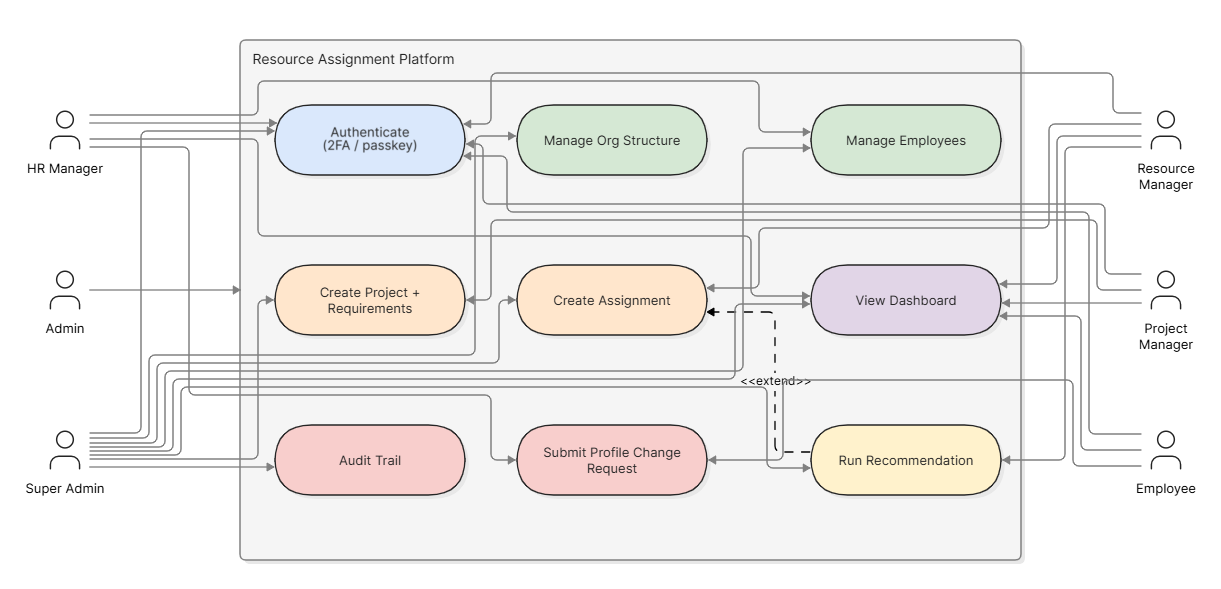
\includegraphics[width=0.95\textwidth]{figures/fig-uc-general.png}
  \caption{Use Case Diagram --- System Actors and Use Cases}
  \label{fig:uc-general}
\end{figure}

\subsection{Codification}
In order to identify unambiguously and in a human-readable way the entities manipulated by the system, a systematic codification was defined. Each business entity receives a code following the format \texttt{PREFIX-N[XX]-[YY]}, where \texttt{PREFIX} identifies the type of the entity, \texttt{N[XX]} is its sequential number within the type, and \texttt{[YY]} is the two-digit year of creation. The code is generated automatically when the entity is created and is guaranteed unique. Table~\ref{tab:codification} summarizes the codification rules applied by the platform.

\begin{table}[H]
  \centering
  \caption{Codification of the business entities}
  \label{tab:codification}
  \begin{tabularx}{\textwidth}{|p{4cm}|X|p{3cm}|}
    \hline
    \rowcolor{tableheader}
    \textcolor{white}{\textbf{Element}} & \textcolor{white}{\textbf{Signification}} & \textcolor{white}{\textbf{Example}} \\
    \hline
    Employee & \texttt{EMPL}-\texttt{N[XX]}-\texttt{[YY]} & EMPL-N03-25 \\ \hline
    Department & \texttt{DEPT}-\texttt{N[XX]}-\texttt{[YY]} & DEPT-N02-25 \\ \hline
    Team & \texttt{TEAM}-\texttt{N[XX]}-\texttt{[YY]} & TEAM-N04-25 \\ \hline
    Position & \texttt{POS}-\texttt{N[XX]}-\texttt{[YY]} & POS-N01-25 \\ \hline
    Location & \texttt{LOC}-\texttt{N[XX]}-\texttt{[YY]} & LOC-N03-25 \\ \hline
    Project & \texttt{PROJ}-\texttt{N[XX]}-\texttt{[YY]} & PROJ-N07-25 \\ \hline
    Skill & \texttt{SKILL}-\texttt{N[XX]}-\texttt{[YY]} & SKILL-N01-25 \\ \hline
    Certification & \texttt{CERT}-\texttt{N[XX]}-\texttt{[YY]} & CERT-N05-25 \\ \hline
    Assignment & \texttt{ASG}-\texttt{N[XX]}-\texttt{[YY]} & ASG-N12-25 \\ \hline
  \end{tabularx}
\end{table}

\subsection{Rules of Management (R\`egles de Gestion)}
The rules of management express, in natural language, the business constraints that the system must enforce independently of any technical choice. Table~\ref{tab:regles} lists the principal rules applied by the platform; several of them are enforced at the database level in addition to the application layer.

\begin{table}[H]
  \centering
  \caption{Principal rules of management (cardinalities and constraints)}
  \label{tab:regles}
  \begin{tabularx}{\textwidth}{|p{1.2cm}|X|}
    \hline
    \rowcolor{tableheader}
    \textcolor{white}{\textbf{Rule}} & \textcolor{white}{\textbf{Description}} \\
    \hline
    RG01 & A User is linked to at most one Employee; the foreign key \texttt{employees.user\_id} is protected by RESTRICT on delete. \\ \hline
    RG02 & A Business Unit contains one-to-many Departments; a Department contains one-to-many Teams; a Department has zero or one ParentDepartment. \\ \hline
    RG03 & An Employee belongs to one Department, one Team, one Position, one Location and zero or one Manager (self-reference). \\ \hline
    RG04 & A Skill, a Certification and a Language are linked many-to-many to Employees through pivot tables (\texttt{employee\_skills}, \texttt{employee\_certifications}, \texttt{employee\_languages}) carrying the proficiency level (1--5). \\ \hline
    RG05 & An Employee has one-to-many Availability records and one-to-many Workload records; all percentages are constrained between 0 and 100. \\ \hline
    RG06 & A Project has one-to-many Requirements (typed); it links many-to-many to Skills, Certifications and Languages through pivots carrying a minimum level and a weight. \\ \hline
    RG07 & An Assignment concerns exactly one Project; it links many-to-many to Employees (\texttt{assignment\_members}) and to Teams (\texttt{assignment\_teams}). \\ \hline
    RG08 & At most one Approved or Active assignment exists per Project (enforced by a partial unique index). \\ \hline
    RG09 & Every status transition of an Assignment is recorded in \texttt{assignment\_status\_history} with the actor and the reason. \\ \hline
    RG10 & An Employee generates zero or more ProfileChangeRequests; a User (reviewer) validates zero or more of them before the changes are applied. \\ \hline
    RG11 & A RecommendationRun produces an ordered list of Recommendations (rank, score); a Project can receive several candidate evaluations. \\ \hline
  \end{tabularx}
\end{table}

\section{Use Case Descriptions}

\subsection{Use Case 1: Authentication with 2FA and Passkeys}

\begin{usecasetable}{Use Case: Authentication with 2FA and Passkeys}
\ucfield{Title}{Authentication with 2FA and Passkeys}
\ucfield{Actors}{All Users}
\ucfield{Description}{User logs in with email/password. If 2FA is enabled, a TOTP code or recovery code is required. Passkeys offer passwordless login via WebAuthn.}
\ucfield{Pre-conditions}{User has valid account. 2FA may be enabled. Passkey may be registered.}
\ucfield{Post-conditions}{User is authenticated and redirected to dashboard or admin panel based on role.}
\ucfield{Main Flow}{
  1. User navigates to login page and enters email and password\\
  2. System validates credentials via Laravel Fortify\\
  3. If 2FA is enabled, system displays TOTP challenge\\
  4. User enters 6-digit code or recovery code\\
  5. System verifies code and creates authenticated session\\
}
\ucfield{Alternative Flow}{Passkey login: system triggers WebAuthn challenge, user verifies via biometric/security key, session is created without password.}
\end{usecasetable}

\begin{figure}[htbp]
  \centering
  \resizebox{!}{0.4\textheight}{% activity-auth.tex — Fig 3.2 : Activity diagram — Authentication
\begin{tikzpicture}[
  >=Stealth,
  node distance=0.6cm and 1.2cm,
  act/.style={draw, rounded corners=3pt, minimum width=4.2cm, minimum height=0.75cm, align=center, font=\small},
  err/.style={draw, rounded corners=3pt, minimum width=2.4cm, minimum height=0.75cm, align=center, font=\small},
  dec/.style={draw, diamond, aspect=2.1, inner sep=2pt, align=center, font=\scriptsize},
  start/.style={circle, fill=black, inner sep=0pt, minimum size=3mm},
  endnode/.style={circle, draw, thick, inner sep=0pt, minimum size=3mm}
]
  % --- Central Flow Nodes ---
  \node[start] (s) {};
  \node[act, below=0.55cm of s] (a1) {Open login page};
  \node[act, below=0.55cm of a1] (a2) {Enter email and password};
  \node[act, below=0.55cm of a2] (a3) {Validate via Fortify};
  \node[dec, below=0.55cm of a3] (d1) {Valid?};
  \node[dec, below=0.65cm of d1] (d2) {2FA enabled?};
  \node[act, below=0.65cm of d2] (a5) {TOTP / recovery code};
  \node[dec, below=0.55cm of a5] (d3) {Code OK?};
  \node[act, below=0.65cm of d3] (a7) {Create session;\\ redirect by role};
  \node[endnode, below=0.55cm of a7] (e) {};

  % --- Error / Rejection Nodes (Left Column) ---
  \node[err, left=1.2cm of d1] (a4) {Show error};
  \node[err, left=1.2cm of d3] (a6) {Reject};

  % --- Main Spine Connectors ---
  \draw[-{Stealth}] (s) -- (a1);
  \draw[-{Stealth}] (a1) -- (a2);
  \draw[-{Stealth}] (a2) -- (a3);
  \draw[-{Stealth}] (a3) -- (d1);
  \draw[-{Stealth}] (d1) -- node[right, font=\scriptsize] {Yes} (d2);
  \draw[-{Stealth}] (d2) -- node[right, font=\scriptsize] {Yes} (a5);
  \draw[-{Stealth}] (a5) -- (d3);
  \draw[-{Stealth}] (d3) -- node[right, font=\scriptsize] {Yes} (a7);
  \draw[-{Stealth}] (a7) -- (e);

  % --- Rejection Branches & Return Bus (Left) ---
  \draw[-{Stealth}] (d1) -- node[above, font=\scriptsize] {No} (a4);
  \draw[-{Stealth}] (d3) -- node[above, font=\scriptsize] {No} (a6);

  \coordinate (bus) at ([xshift=-0.6cm]a4.west);
  \draw (a6.west) -- (bus |- a6.west);
  \draw (a4.west) -- (bus |- a4.west);
  \draw[-{Stealth}] (bus |- a6.west) -- (bus |- a1.west) -- (a1.west);

  % --- 2FA Bypass (Right) ---
  \coordinate (bypass) at ([xshift=0.9cm]a5.east);
  \draw[-{Stealth}] (d2.east) -- node[above, font=\scriptsize] {No} (bypass |- d2.east) |- (a7.east);

\end{tikzpicture}}
  \caption{Activity diagram --- Authentication with 2FA and passkeys}
  \label{fig:activity-auth}
\end{figure}

\subsection{Use Case 2: Manage Organization Structure}

\begin{usecasetable}{Use Case: Manage Organization Structure}
\ucfield{Title}{Manage Organization Structure}
\ucfield{Actors}{Super Admin, Admin}
\ucfield{Description}{Admin creates and manages business units, departments, teams, positions, and locations with hierarchical relationships (departments belong to business units, teams belong to departments, positions belong to teams).}
\ucfield{Pre-conditions}{User authenticated with appropriate permissions.}
\ucfield{Post-conditions}{Organization structure is updated with new or modified entities.}
\ucfield{Main Flow}{
  1. Admin navigates to organization section in Filament panel\\
  2. Admin selects entity type (business unit, department, team, position, or location)\\
  3. System displays list view with search, filters, and sort\\
  4. Admin creates or edits entity with form validation\\
  5. System saves changes with audit log entry\\
}
\ucfield{Alternative Flow}{Invalid parent reference triggers validation error. Deleting a parent with children triggers restrictOnDelete constraint.}
\end{usecasetable}

\begin{figure}[htbp]
  \centering
  \resizebox{!}{0.4\textheight}{% activity-org.tex — Fig 3.3 : Activity diagram — Manage organization structure
\begin{tikzpicture}[
  >=Stealth,
  node distance=0.55cm and 1.4cm,
  act/.style={draw, rounded corners=3pt, minimum width=4.8cm, minimum height=0.75cm, align=center, font=\small},
  err/.style={draw, rounded corners=3pt, minimum width=2.8cm, minimum height=0.75cm, align=center, font=\small},
  dec/.style={draw, diamond, aspect=2.1, inner sep=2pt, align=center, font=\scriptsize},
  start/.style={circle, fill=black, inner sep=0pt, minimum size=3mm},
  endnode/.style={circle, draw, thick, inner sep=0pt, minimum size=3mm}
]
  % --- Central Flow Nodes ---
  \node[start] (s) {};
  \node[act, below=0.55cm of s] (a1) {Open Org section in Filament};
  \node[act, below=0.55cm of a1] (a2) {Select entity (BU/Dept/Team/Pos/Loc)};
  \node[act, below=0.55cm of a2] (a3) {Create or edit entity};
  \node[dec, below=0.55cm of a3] (d1) {Valid parent?};
  \node[act, below=0.65cm of d1] (a5) {Save change};
  \node[act, below=0.55cm of a5] (a6) {Write audit log entry};
  \node[endnode, below=0.55cm of a6] (e) {};

  % --- Error / Rejection Node (Left) ---
  \node[err, left=1.4cm of d1] (a4) {Validation error};

  % --- Connectors ---
  \draw[-{Stealth}] (s) -- (a1);
  \draw[-{Stealth}] (a1) -- (a2);
  \draw[-{Stealth}] (a2) -- (a3);
  \draw[-{Stealth}] (a3) -- (d1);
  \draw[-{Stealth}] (d1) -- node[above, font=\scriptsize] {No} (a4);
  \draw[-{Stealth}] (a4.west) -- ++(-0.6,0) |- (a2.west);
  \draw[-{Stealth}] (d1) -- node[right, font=\scriptsize] {Yes} (a5);
  \draw[-{Stealth}] (a5) -- (a6);
  \draw[-{Stealth}] (a6) -- (e);
\end{tikzpicture}}
  \caption{Activity diagram --- Manage organization structure}
  \label{fig:activity-org}
\end{figure}

\subsection{Use Case 3: Create and Manage Employees}

\begin{usecasetable}{Use Case: Create and Manage Employees}
\ucfield{Title}{Create and Manage Employees}
\ucfield{Actors}{Super Admin, Admin, HR Manager}
\ucfield{Description}{HR creates employee profiles linked to organizational entities, then enriches with skills, certifications, languages, availability status, and workload data.}
\ucfield{Pre-conditions}{User authenticated with employee management permissions. Organizational structure exists.}
\ucfield{Post-conditions}{Employee profile is created with complete profile data.}
\ucfield{Main Flow}{
  1. HR navigates to employee management in Filament panel\\
  2. HR creates new employee with personal info, department, position, location, employment type and status\\
  3. HR adds skills with proficiency levels (beginner/intermediate/advanced/native)\\
  4. HR adds certifications with verification status (pending/verified/rejected/expired)\\
  5. HR adds languages with proficiency levels\\
  6. HR sets availability status (available/partially available/unavailable/on leave) and workload percentages\\
}
\ucfield{Alternative Flow}{Editing employee linked to active assignment triggers warning. Soft-deleting employee preserves assignment history.}
\end{usecasetable}

\begin{figure}[htbp]
  \centering
  \resizebox{!}{0.4\textheight}{% activity-employee.tex — Fig 3.4 : Activity diagram — Create and manage employees
\begin{tikzpicture}[
  >=Stealth, node distance=0.9cm and 1.6cm,
  act/.style={draw, rounded corners=3pt, minimum width=4.6cm, minimum height=0.8cm, align=center, font=\small},
  dec/.style={draw, diamond, aspect=2.1, inner sep=1pt, align=center, font=\scriptsize},
  start/.style={circle, fill=black, inner sep=0pt, minimum size=3mm},
  endnode/.style={circle, draw, thick, inner sep=0pt, minimum size=3mm}
]
\node[start] (s) {};
\node[act, below=0.8cm of s] (a1) {Open Employee resource in Filament};
\node[act, below=0.8cm of a1] (a2) {Enter personal info + org links};
\node[act, below=0.8cm of a2] (a3) {Add skills / certs / languages};
\node[act, below=0.8cm of a3] (a4) {Set availability + workload \%};
\node[dec, below=0.8cm of a4] (d1) {Valid profile?};
\node[act, below left=1.1cm and 0.8cm of d1] (a5) {Fix errors};
\node[act, below=0.85cm of d1] (a6) {Save employee};
\node[act, below=0.8cm of a6] (a7) {Audit log + notify};
\node[endnode, below=0.8cm of a7] (e) {};
\draw[-{Stealth}] (s) -- (a1);
\draw[-{Stealth}] (a1) -- (a2);
\draw[-{Stealth}] (a2) -- (a3);
\draw[-{Stealth}] (a3) -- (a4);
\draw[-{Stealth}] (a4) -- (d1);
\draw[-{Stealth}] (d1) -- node[above, font=\scriptsize]{No} (a5);
\draw[-{Stealth}] (a5.south) -- ++(0,-0.5) -| (a2.west);
\draw[-{Stealth}] (d1) -- node[left, font=\scriptsize]{Yes} (a6);
\draw[-{Stealth}] (a6) -- (a7);
\draw[-{Stealth}] (a7) -- (e);
\end{tikzpicture}}
  \caption{Activity diagram --- Create and manage employees}
  \label{fig:activity-employee}
\end{figure}

\subsection{Use Case 4: Create Project with Requirements}

\begin{usecasetable}{Use Case: Create Project with Requirements}
\ucfield{Title}{Create Project with Requirements}
\ucfield{Actors}{Super Admin, Admin, Project Manager}
\ucfield{Description}{Project manager creates a project, defines category, assignment mode, priority, dates, confidentiality level, and adds typed requirements (skills, certifications, languages, experience, position, department, location, availability).}
\ucfield{Pre-conditions}{User authenticated with project management permissions. Project categories exist.}
\ucfield{Post-conditions}{Project is created in Draft status with defined requirements.}
\ucfield{Main Flow}{
  1. PM navigates to project management in Filament panel\\
  2. PM creates new project with name, description, category, assignment mode, priority, status, dates, and confidentiality level\\
  3. System saves project in Draft status\\
  4. PM adds project requirements (skill, certification, language, or other requirement types) with minimum level and weight\\
  5. System validates and stores requirements\\
}
\ucfield{Alternative Flow}{Changing assignment mode after assignment exists triggers validation. Status transitions follow: Draft $\rightarrow$ Submitted $\rightarrow$ Under Review $\rightarrow$ Staffing $\rightarrow$ Assigned $\rightarrow$ In Progress $\rightarrow$ Completed.}
\end{usecasetable}

\begin{figure}[htbp]
  \centering
  \resizebox{!}{0.4\textheight}{% activity-project.tex — Fig 3.5 : Activity diagram — Create project with requirements
\begin{tikzpicture}[
  >=Stealth, node distance=0.9cm and 1.6cm,
  act/.style={draw, rounded corners=3pt, minimum width=4.6cm, minimum height=0.8cm, align=center, font=\small},
  dec/.style={draw, diamond, aspect=2.1, inner sep=1pt, align=center, font=\scriptsize},
  start/.style={circle, fill=black, inner sep=0pt, minimum size=3mm},
  endnode/.style={circle, draw, thick, inner sep=0pt, minimum size=3mm}
]
\node[start] (s) {};
\node[act, below=0.8cm of s] (a1) {Open Project resource in Filament};
\node[act, below=0.8cm of a1] (a2) {Define metadata (category, mode, dates)};
\node[act, below=0.8cm of a2] (a3) {Save project (Draft)};
\node[act, below=0.8cm of a3] (a4) {Add typed requirements};
\node[dec, below=0.8cm of a4] (d1) {Complete?};
\node[act, below left=1.1cm and 0.8cm of d1] (a5) {Continue editing};
\node[act, below=0.85cm of d1] (a6) {Submit project};
\node[act, below=0.8cm of a6] (a7) {Set status Under Review};
\node[endnode, below=0.8cm of a7] (e) {};
\draw[-{Stealth}] (s) -- (a1);
\draw[-{Stealth}] (a1) -- (a2);
\draw[-{Stealth}] (a2) -- (a3);
\draw[-{Stealth}] (a3) -- (a4);
\draw[-{Stealth}] (a4) -- (d1);
\draw[-{Stealth}] (d1) -- node[above, font=\scriptsize]{No} (a5);
\draw[-{Stealth}] (a5.south) -- ++(0,-0.5) -| (a4.west);
\draw[-{Stealth}] (d1) -- node[left, font=\scriptsize]{Yes} (a6);
\draw[-{Stealth}] (a6) -- (a7);
\draw[-{Stealth}] (a7) -- (e);
\end{tikzpicture}}
  \caption{Activity diagram --- Create project with requirements}
  \label{fig:activity-project}
\end{figure}

\subsection{Use Case 5: Create Assignment with Status Workflow}

\begin{usecasetable}{Use Case: Create Assignment with Status Workflow}
\ucfield{Title}{Create Assignment with Status Workflow}
\ucfield{Actors}{Super Admin, Admin, Resource Manager}
\ucfield{Description}{Resource manager creates an assignment linking employees or teams to a project, then progresses through status machine: Pending $\rightarrow$ Approved $\rightarrow$ Active $\rightarrow$ Completed (or Rejected/Cancelled at various stages).}
\ucfield{Pre-conditions}{User authenticated with assignment permissions. Project exists. Employees are active.}
\ucfield{Post-conditions}{Assignment is created and status history is recorded. Single-active-per-project rule is enforced.}
\ucfield{Main Flow}{
  1. RM navigates to assignment management in Filament panel\\
  2. RM creates new assignment for a project with assignment type (employee/team/department)\\
  3. System validates no current approved or active assignment exists for the project (partial unique index)\\
  4. RM assigns members (employees) with allocation percentage, responsibility, and dates\\
  5. RM assigns teams if applicable\\
  6. Assignment starts in Pending status\\
  7. Approver transitions assignment to Approved (records approver and timestamp)\\
  8. RM activates the assignment (transitions to Active)\\
  9. Upon completion, RM marks assignment Completed (triggers left\_at date on all members)\\
}
\ucfield{Alternative Flow}{Transition from Pending to Rejected or Cancelled records reason in status history. Cancellation allowed from Pending, Approved, or Active status only. DomainException thrown for invalid transitions.}
\end{usecasetable}

\begin{figure}[htbp]
  \centering
  \resizebox{!}{0.4\textheight}{% activity-assignment.tex — Fig 3.6 : Activity diagram — Assignment status workflow
\begin{tikzpicture}[
  >=Stealth,
  node distance=0.48cm and 1.4cm,
  act/.style={draw, rounded corners=3pt, minimum width=4.8cm, minimum height=0.72cm, align=center, font=\small},
  err/.style={draw, rounded corners=3pt, minimum width=3.2cm, minimum height=0.72cm, align=center, font=\small},
  dec/.style={draw, diamond, aspect=2.1, inner sep=2pt, align=center, font=\scriptsize},
  start/.style={circle, fill=black, inner sep=0pt, minimum size=3mm},
  endnode/.style={circle, draw, thick, inner sep=0pt, minimum size=3mm}
]
  % --- Central Flow Nodes ---
  \node[start] (s) {};
  \node[act, below=0.48cm of s] (a1) {Create assignment for project};
  \node[act, below=0.48cm of a1] (a2) {Add members/teams + allocations};
  \node[dec, below=0.48cm of a2] (d0) {Single active\\assignment?};
  \node[act, below=0.55cm of d0] (a3) {Save as Pending};
  \node[dec, below=0.48cm of a3] (d1) {Approve?};
  \node[act, below=0.55cm of d1] (a5) {Approved (rec. approver)};
  \node[act, below=0.48cm of a5] (a6) {Activate};
  \node[act, below=0.48cm of a6] (a7) {Complete (set left\_at)};
  \node[endnode, below=0.48cm of a7] (e) {};

  % --- Rejection / Blocking Nodes (Left Column) ---
  \node[err, left=1.4cm of d0] (a0) {Block (violation)};
  \node[err, left=1.4cm of d1] (a4) {Rejected / Cancelled};

  % --- Main Connectors ---
  \draw[-{Stealth}] (s) -- (a1);
  \draw[-{Stealth}] (a1) -- (a2);
  \draw[-{Stealth}] (a2) -- (d0);
  \draw[-{Stealth}] (d0) -- node[above, font=\scriptsize] {No} (a0);
  \draw[-{Stealth}] (a0.west) -- ++(-0.6,0) |- (a1.west);
  \draw[-{Stealth}] (d0) -- node[right, font=\scriptsize] {Yes} (a3);
  \draw[-{Stealth}] (a3) -- (d1);
  \draw[-{Stealth}] (d1) -- node[above, font=\scriptsize] {No} (a4);
  \draw[-{Stealth}] (d1) -- node[right, font=\scriptsize] {Yes} (a5);
  \draw[-{Stealth}] (a5) -- (a6);
  \draw[-{Stealth}] (a6) -- (a7);
  \draw[-{Stealth}] (a7) -- (e);
\end{tikzpicture}}
  \caption{Activity diagram --- Assignment status workflow}
  \label{fig:activity-assignment}
\end{figure}

\subsection{Use Case 6: View Dashboard Analytics}

\begin{usecasetable}{Use Case: View Dashboard Analytics}
\ucfield{Title}{View Dashboard Analytics}
\ucfield{Actors}{All authenticated users}
\ucfield{Description}{Dashboard displays key metrics: total employees by department, workload vs availability chart, projects by status, projects needing staffing, over-allocated employees, expiring certifications, and recent activity log.}
\ucfield{Pre-conditions}{User authenticated.}
\ucfield{Post-conditions}{Dashboard displays current state of organization and assignments.}
\ucfield{Main Flow}{
  1. User navigates to dashboard (Filament panel for admin users, public dashboard for regular users)\\
  2. System loads StatsOverview widget (total counts)\\
  3. System loads EmployeesByDepartmentChart (bar chart)\\
  4. System loads AllocationVsAvailabilityChart (grouped bar: workload vs availability per department)\\
  5. System loads ProjectsByStatusChart (doughnut chart)\\
  6. System loads alert tables: ProjectsNeedingStaffing, OverAllocatedEmployees, ExpiringCertifications\\
  7. System loads RecentActivityTable (audit log entries)\\
}
\ucfield{Alternative Flow}{Empty data states show placeholder messages. Charts are rendered client-side via Filament ChartWidget.}
\end{usecasetable}

\begin{figure}[htbp]
  \centering
  \resizebox{!}{0.4\textheight}{% activity-dashboard.tex — Fig 3.7 : Activity diagram — View dashboard analytics
\begin{tikzpicture}[
  >=Stealth,
  node distance=0.55cm and 1.4cm,
  act/.style={draw, rounded corners=3pt, minimum width=4.8cm, minimum height=0.75cm, align=center, font=\small},
  alt/.style={draw, rounded corners=3pt, minimum width=2.4cm, minimum height=0.75cm, align=center, font=\small},
  dec/.style={draw, diamond, aspect=2.1, inner sep=2pt, align=center, font=\scriptsize},
  start/.style={circle, fill=black, inner sep=0pt, minimum size=3mm},
  endnode/.style={circle, draw, thick, inner sep=0pt, minimum size=3mm}
]
  % --- Central Flow Nodes ---
  \node[start] (s) {};
  \node[act, below=0.55cm of s] (a1) {Authenticate and open dashboard};
  \node[act, below=0.55cm of a1] (a2) {Load stat cards};
  \node[act, below=0.55cm of a2] (a3) {Load 3 charts};
  \node[act, below=0.55cm of a3] (a4) {Load alert tables};
  \node[dec, below=0.55cm of a4] (d1) {Over-allocation?};
  \node[act, below=0.65cm of d1] (a6) {Show audit activity feed};
  \node[endnode, below=0.55cm of a6] (e) {};

  % --- Alert Branch (Left) ---
  \node[alt, left=1.4cm of d1] (a5) {Show alert};

  % --- Connectors ---
  \draw[-{Stealth}] (s) -- (a1);
  \draw[-{Stealth}] (a1) -- (a2);
  \draw[-{Stealth}] (a2) -- (a3);
  \draw[-{Stealth}] (a3) -- (a4);
  \draw[-{Stealth}] (a4) -- (d1);
  \draw[-{Stealth}] (d1) -- node[above, font=\scriptsize] {Yes} (a5);
  \draw[-{Stealth}] (a5.south) |- (a6.west);
  \draw[-{Stealth}] (d1) -- node[right, font=\scriptsize] {No} (a6);
  \draw[-{Stealth}] (a6) -- (e);
\end{tikzpicture}}
  \caption{Activity diagram --- View dashboard analytics}
  \label{fig:activity-dashboard}
\end{figure}

\subsection{Use Case 7: Audit Trail}

\begin{usecasetable}{Use Case: Audit Trail}
\ucfield{Title}{Audit Trail}
\ucfield{Actors}{Super Admin, Admin}
\ucfield{Description}{Every assignment action (created, approved, activated, completed, rejected, cancelled) is recorded in audit\_logs with actor ID, action, auditable type and ID, old/new values, IP address, and user agent.}
\ucfield{Pre-conditions}{AuditService is injected into AssignmentService.}
\ucfield{Post-conditions}{Audit log entry is created for every state transition.}
\ucfield{Main Flow}{
  1. Assignment state transition occurs (e.g., approve)\\
  2. AssignmentService calls AuditService.assignmentTransition()\\
  3. AuditService creates AuditLog record with action, old\_values, new\_values, IP, user\_agent\\
  4. Record is persisted to audit\_logs table\\
}
\ucfield{Alternative Flow}{Manual log entries can be created via AuditService.log() for any model and action.}
\end{usecasetable}

\begin{figure}[htbp]
  \centering
  \resizebox{!}{0.4\textheight}{% activity-audit.tex — Fig 3.8 : Activity diagram — Audit trail capture
\begin{tikzpicture}[
  >=Stealth,
  node distance=0.52cm and 1.4cm,
  act/.style={draw, rounded corners=3pt, minimum width=4.8cm, minimum height=0.72cm, align=center, font=\small},
  pr/.style={draw, rounded corners=3pt, minimum width=3.4cm, minimum height=0.72cm, align=center, font=\small, dashed},
  dec/.style={draw, diamond, aspect=2.1, inner sep=2pt, align=center, font=\scriptsize},
  start/.style={circle, fill=black, inner sep=0pt, minimum size=3mm},
  endnode/.style={circle, draw, thick, inner sep=0pt, minimum size=3mm}
]
  % --- Central Flow Nodes ---
  \node[start] (s) {};
  \node[act, below=0.5cm of s] (a1) {Action performed on entity};
  \node[act, below=0.5cm of a1] (a2) {Event reaches observer / AuditService};
  \node[dec, below=0.5cm of a2] (d1) {Trigger tracked?};
  \node[act, below=0.65cm of d1] (a4) {Serialize old / new values};
  \node[act, below=0.5cm of a4] (a5) {Store audit\_logs row};
  \node[act, below=0.5cm of a5] (a6) {Link to actor + IP + user-agent};
  \node[act, below=0.5cm of a6] (a7) {Refresh audit dashboard feed};
  \node[endnode, below=0.5cm of a7] (e) {};

  % --- Non-tracked Branch (Left) ---
  \node[pr, left=1.4cm of d1] (a3) {Notification only, no log};

  % --- Connectors ---
  \draw[-{Stealth}] (s) -- (a1);
  \draw[-{Stealth}] (a1) -- (a2);
  \draw[-{Stealth}] (a2) -- (d1);
  \draw[-{Stealth}] (d1) -- node[above, font=\scriptsize] {No} (a3);
  \draw[-{Stealth}] (d1) -- node[right, font=\scriptsize] {Yes} (a4);
  \draw[-{Stealth}] (a4) -- (a5);
  \draw[-{Stealth}] (a5) -- (a6);
  \draw[-{Stealth}] (a6) -- (a7);
  \draw[-{Stealth}] (a7) -- (e);
\end{tikzpicture}}
  \caption{Activity diagram --- Audit trail}
  \label{fig:activity-audit}
\end{figure}

\subsection{Use Case 8: Run Recommendation for Staffing}

\begin{usecasetable}{Use Case: Run Recommendation for Staffing}
\ucfield{Title}{Run Recommendation for Staffing}
\ucfield{Actors}{Super Admin, Admin, Resource Manager}
\ucfield{Description}{The system ranks the candidate employees of a project against its typed requirements and produces an ordered recommendation list with scores. The recommendation can operate in three modes: employee, team, or department.}
\ucfield{Pre-conditions}{User authenticated with recommendation permissions. The project exists in the Staffing state and carries typed requirements.}
\ucfield{Post-conditions}{A RecommendationRun is persisted together with the ranked Recommendations; the ordered list is displayed to the resource manager.}
\ucfield{Main Flow}{
  1. RM opens a project in the Staffing state and selects ``Run recommendation''\\
  2. RM chooses the mode (employee, team, or department)\\
  3. The system evaluates every candidate against the weighted typed requirements (skill, certification, language, experience, position, department, location, availability)\\
  4. The candidates are scored and sorted in descending order\\
  5. The system persists the RecommendationRun and the recommendations, then displays the ranked list\\
}
\ucfield{Alternative Flow}{If no candidate satisfies the minimum coverage, an empty result is displayed with an explanatory message.}
\end{usecasetable}

\begin{figure}[htbp]
  \centering
  \resizebox{!}{0.4\textheight}{% activity-recommendation.tex — Fig 3.10 : Activity diagram — Run recommendation for staffing
\begin{tikzpicture}[
  >=Stealth,
  node distance=0.48cm and 1.4cm,
  act/.style={draw, rounded corners=3pt, minimum width=4.8cm, minimum height=0.70cm, align=center, font=\small},
  err/.style={draw, rounded corners=3pt, minimum width=2.8cm, minimum height=0.70cm, align=center, font=\small},
  dec/.style={draw, diamond, aspect=2.1, inner sep=2pt, align=center, font=\scriptsize},
  start/.style={circle, fill=black, inner sep=0pt, minimum size=3mm},
  endnode/.style={circle, draw, thick, inner sep=0pt, minimum size=3mm}
]
  % --- Central Flow Nodes ---
  \node[start] (s) {};
  \node[act, below=0.45cm of s] (a1) {Open project / recommendation run};
  \node[act, below=0.45cm of a1] (a2) {Choose mode (employee/team/dept)};
  \node[act, below=0.45cm of a2] (a3) {Evaluate candidates vs requirements};
  \node[act, below=0.45cm of a3] (a4) {Exclude ineligible employees};
  \node[act, below=0.45cm of a4] (a5) {Score and rank candidates};
  \node[act, below=0.45cm of a5] (a6) {Store run + recommendations};
  \node[dec, below=0.45cm of a6] (d1) {Create assignment?};
  \node[act, below=0.60cm of d1] (a8) {Approve top match + attach};
  \node[endnode, below=0.45cm of a8] (e) {};

  % --- Non-assignment Branch (Left) ---
  \node[err, left=1.4cm of d1] (a7) {End (keep ranking)};

  % --- Connectors ---
  \draw[-{Stealth}] (s) -- (a1);
  \draw[-{Stealth}] (a1) -- (a2);
  \draw[-{Stealth}] (a2) -- (a3);
  \draw[-{Stealth}] (a3) -- (a4);
  \draw[-{Stealth}] (a4) -- (a5);
  \draw[-{Stealth}] (a5) -- (a6);
  \draw[-{Stealth}] (a6) -- (d1);
  \draw[-{Stealth}] (d1) -- node[above, font=\scriptsize] {No} (a7);
  \draw[-{Stealth}] (d1) -- node[right, font=\scriptsize] {Yes} (a8);
  \draw[-{Stealth}] (a8) -- (e);
\end{tikzpicture}}
  \caption{Activity diagram --- Run recommendation for staffing}
  \label{fig:activity-recommendation}
\end{figure}

\subsection{Use Case 9: Submit and Approve Profile Change Requests}

\begin{usecasetable}{Use Case: Submit and Approve Profile Change Requests}
\ucfield{Title}{Submit and Approve Profile Change Requests}
\ucfield{Actors}{Employee (submits), HR Manager / Admin (approves)}
\ucfield{Description}{Through the self-service portal, an employee requests updates to their own profile (contact, skills, availability, and so on). The changes are applied only after the approval of an HR manager, keeping the referential under control.}
\ucfield{Pre-conditions}{The employee is authenticated on the portal and the requested fields are editable.}
\ucfield{Post-conditions}{The approved changes are applied to the employee profile and the whole flow is recorded in the audit trail.}
\ucfield{Main Flow}{
  1. The employee opens the profile page of the portal\\
  2. The employee submits a change request with the new values and a reason\\
  3. The system stores a ProfileChangeRequest in the Pending state\\
  4. An HR manager reviews the request\\
  5. If approved, the system applies the changes and records the audit; otherwise it rejects the request with a reason\\
}
\ucfield{Alternative Flow}{The employee may cancel an own request that has not yet been reviewed.}
\end{usecasetable}

\begin{figure}[htbp]
  \centering
  \resizebox{!}{0.4\textheight}{% activity-profile.tex — Fig 3.9 : Activity diagram — Submit and approve profile change requests
\begin{tikzpicture}[
  >=Stealth, node distance=0.9cm and 1.6cm,
  act/.style={draw, rounded corners=3pt, minimum width=4.8cm, minimum height=0.8cm, align=center, font=\small},
  dec/.style={draw, diamond, aspect=2.1, inner sep=1pt, align=center, font=\scriptsize},
  start/.style={circle, fill=black, inner sep=0pt, minimum size=3mm},
  endnode/.style={circle, draw, thick, inner sep=0pt, minimum size=3mm}
]
\node[start] (s) {};
\node[act, below=0.8cm of s] (a1) {Employee opens portal /portal};
\node[act, below=0.8cm of a1] (a2) {Chooses a profile section};
\node[act, below=0.8cm of a2] (a3) {Submits change request};
\node[act, below=0.8cm of a3] (a4) {Snapshot previous values (Pending)};
\node[act, below=0.8cm of a4] (a5) {Notify HR reviewers};
\node[dec, below=0.8cm of a5] (d1) {HR approves?};
\node[act, below left=1.1cm and 0.6cm of d1] (a6) {Reject (note)};
\node[act, below=0.85cm of d1] (a7) {Apply change to profile};
\node[act, below=0.8cm of a7] (a8) {Notify employee};
\node[endnode, below=0.8cm of a8] (e) {};
\draw[-{Stealth}] (s) -- (a1);
\draw[-{Stealth}] (a1) -- (a2);
\draw[-{Stealth}] (a2) -- (a3);
\draw[-{Stealth}] (a3) -- (a4);
\draw[-{Stealth}] (a4) -- (a5);
\draw[-{Stealth}] (a5) -- (d1);
\draw[-{Stealth}] (d1) -- node[above, font=\scriptsize]{No} (a6);
\draw[-{Stealth}] (d1) -- node[left, font=\scriptsize]{Yes} (a7);
\draw[-{Stealth}] (a7) -- (a8);
\draw[-{Stealth}] (a8) -- (e);
\end{tikzpicture}}
  \caption{Activity diagram --- Submit and approve profile change requests}
  \label{fig:activity-profile}
\end{figure}

\section{Dynamic Study --- Sequence Diagrams}

The sequence diagrams below describe the exchange of messages between the actors and the application objects for the main scenarios of the platform. Figure~\ref{fig:seq-auth} details the authentication, Figure~\ref{fig:seq-org} the management of the organization, Figure~\ref{fig:seq-employee} the creation of an employee, Figure~\ref{fig:seq-project} the creation of a project, Figure~\ref{fig:seq-assignment} the assignment lifecycle, Figure~\ref{fig:seq-dashboard} the display of the dashboard, Figure~\ref{fig:seq-audit} the audit capture, Figure~\ref{fig:seq-portal} the approval of a profile change request, and Figure~\ref{fig:seq-reco} a recommendation run.

\begin{figure}[htbp]
  \centering
  \resizebox{0.98\textwidth}{!}{% sequence-auth.tex — Fig 3.11 : Sequence — Authentication with 2FA/passkeys
\begin{tikzpicture}[>=Stealth, font=\scriptsize]
\def\H{6.4}
\node (u) at (0.6,0) {User};
\node (b) at (3.6,0) {Login Page};
\node (f) at (7.0,0) {Fortify};
\node (d) at (10.4,0) {Database};
\draw[dashed] (u.south) -- (0.6,-\H);
\draw[dashed] (b.south) -- (3.6,-\H);
\draw[dashed] (f.south) -- (7.0,-\H);
\draw[dashed] (d.south) -- (10.4,-\H);
\draw[fill=black!12] (3.45,-0.7) rectangle (3.75,-5.7);
\draw[fill=black!12] (6.85,-1.3) rectangle (7.15,-5.1);
\draw[fill=black!12] (10.25,-1.9) rectangle (10.55,-4.3);
\draw[-{Stealth}] (0.6,-0.8) -- (3.6,-0.8) node[midway,above]{email + password};
\draw[-{Stealth}] (3.6,-1.4) -- (7.0,-1.4) node[midway,above]{validate credentials};
\draw[-{Stealth}] (7.0,-2.0) -- (10.4,-2.0) node[midway,above]{select user + 2FA flag};
\draw[-{Stealth}] (10.4,-2.6) -- (7.0,-2.6) node[midway,above]{result};
\draw[-{Stealth}] (0.6,-3.2) -- (3.6,-3.2) node[midway,above]{if 2FA: TOTP / recovery};
\draw[-{Stealth}] (3.6,-3.8) -- (7.0,-3.8) node[midway,above]{verify code};
\draw[-{Stealth}] (7.0,-4.4) -- (10.4,-4.4) node[midway,above]{create session};
\draw[-{Stealth}] (7.0,-5.0) -- (3.6,-5.0) node[midway,above]{authenticated};
\draw[-{Stealth}] (3.6,-5.6) -- (0.6,-5.6) node[midway,above]{redirect by role};
\end{tikzpicture}}
  \caption{Sequence diagram --- Authentication with 2FA/passkeys}
  \label{fig:seq-auth}
\end{figure}

\begin{figure}[htbp]
  \centering
  \resizebox{0.98\textwidth}{!}{% sequence-org.tex — Fig 3.12 : Sequence — Manage organization structure
\begin{tikzpicture}[>=Stealth, font=\scriptsize]
\def\H{5.6}
\node (m) at (0.6,0) {Manager};
\node (b) at (3.6,0) {Filament UI};
\node (s) at (7.0,0) {OrgService};
\node (d) at (10.4,0) {Database};
\draw[dashed] (m.south) -- (0.6,-\H);
\draw[dashed] (b.south) -- (3.6,-\H);
\draw[dashed] (s.south) -- (7.0,-\H);
\draw[dashed] (d.south) -- (10.4,-\H);
\draw[fill=black!12] (3.45,-0.7) rectangle (3.75,-4.9);
\draw[fill=black!12] (6.85,-1.3) rectangle (7.15,-4.3);
\draw[fill=black!12] (10.25,-1.9) rectangle (10.55,-3.7);
\draw[-{Stealth}] (0.6,-0.8) -- (3.6,-0.8) node[midway,above]{open org section};
\draw[-{Stealth}] (3.6,-1.4) -- (7.0,-1.4) node[midway,above]{create entity};
\draw[-{Stealth}] (7.0,-2.0) -- (10.4,-2.0) node[midway,above]{validate parent FK};
\draw[-{Stealth}] (10.4,-2.6) -- (7.0,-2.6) node[midway,above]{saved};
\draw[-{Stealth}] (7.0,-3.2) -- (10.4,-3.2) node[midway,above]{write audit log};
\draw[-{Stealth}] (7.0,-3.8) -- (3.6,-3.8) node[midway,above]{confirmation};
\draw[-{Stealth}] (3.6,-4.4) -- (0.6,-4.4) node[midway,above]{entity created};
\end{tikzpicture}}
  \caption{Sequence diagram --- Manage organization structure}
  \label{fig:seq-org}
\end{figure}

\begin{figure}[htbp]
  \centering
  \resizebox{0.98\textwidth}{!}{% sequence-employee.tex — Fig 3.13 : Sequence — Create employee
\begin{tikzpicture}[>=Stealth, font=\scriptsize]
\def\H{6.2}
\node (h) at (0.6,0) {HR};
\node (b) at (3.6,0) {Filament UI};
\node (s) at (7.0,0) {EmployeeService};
\node (d) at (10.4,0) {Database};
\draw[dashed] (h.south) -- (0.6,-\H);
\draw[dashed] (b.south) -- (3.6,-\H);
\draw[dashed] (s.south) -- (7.0,-\H);
\draw[dashed] (d.south) -- (10.4,-\H);
\draw[fill=black!12] (3.45,-0.7) rectangle (3.75,-5.5);
\draw[fill=black!12] (6.85,-1.3) rectangle (7.15,-4.9);
\draw[fill=black!12] (10.25,-1.9) rectangle (10.55,-4.3);
\draw[-{Stealth}] (0.6,-0.8) -- (3.6,-0.8) node[midway,above]{open Employee resource};
\draw[-{Stealth}] (3.6,-1.4) -- (7.0,-1.4) node[midway,above]{store(profile)};
\draw[-{Stealth}] (7.0,-2.0) -- (10.4,-2.0) node[midway,above]{insert employee + traits};
\draw[-{Stealth}] (10.4,-2.6) -- (7.0,-2.6) node[midway,above]{ok};
\draw[-{Stealth}] (7.0,-3.2) -- (10.4,-3.2) node[midway,above]{audit log};
\draw[-{Stealth}] (7.0,-3.8) -- (3.6,-3.8) node[midway,above]{saved};
\draw[-{Stealth}] (3.6,-4.4) -- (0.6,-4.4) node[midway,above]{employee created};
\draw[-{Stealth}] (7.0,-5.0) -- (10.4,-5.0) node[midway,above]{notification (optional)};
\end{tikzpicture}}
  \caption{Sequence diagram --- Create employee}
  \label{fig:seq-employee}
\end{figure}

\begin{figure}[htbp]
  \centering
  \resizebox{0.98\textwidth}{!}{% sequence-project.tex — Fig 3.14 : Sequence — Create project with requirements
\begin{tikzpicture}[>=Stealth, font=\scriptsize]
\def\H{6.4}
\node (p) at (0.6,0) {PM};
\node (b) at (3.6,0) {Filament UI};
\node (s) at (7.0,0) {ProjectService};
\node (d) at (10.4,0) {Database};
\draw[dashed] (p.south) -- (0.6,-\H);
\draw[dashed] (b.south) -- (3.6,-\H);
\draw[dashed] (s.south) -- (7.0,-\H);
\draw[dashed] (d.south) -- (10.4,-\H);
\draw[fill=black!12] (3.45,-0.7) rectangle (3.75,-5.7);
\draw[fill=black!12] (6.85,-1.3) rectangle (7.15,-5.0);
\draw[fill=black!12] (10.25,-1.9) rectangle (10.55,-4.4);
\draw[-{Stealth}] (0.6,-0.8) -- (3.6,-0.8) node[midway,above]{open Project resource};
\draw[-{Stealth}] (3.6,-1.4) -- (7.0,-1.4) node[midway,above]{create(project)};
\draw[-{Stealth}] (7.0,-2.0) -- (10.4,-2.0) node[midway,above]{save project};
\draw[-{Stealth}] (10.4,-2.6) -- (7.0,-2.6) node[midway,above]{id};
\draw[-{Stealth}] (3.6,-3.2) -- (7.0,-3.2) node[midway,above]{add requirements};
\draw[-{Stealth}] (7.0,-3.8) -- (10.4,-3.8) node[midway,above]{insert requirements};
\draw[-{Stealth}] (10.4,-4.4) -- (7.0,-4.4) node[midway,above]{ok};
\draw[-{Stealth}] (7.0,-5.0) -- (3.6,-5.0) node[midway,above]{project ready};
\draw[-{Stealth}] (3.6,-5.6) -- (0.6,-5.6) node[midway,above]{requirements saved};
\end{tikzpicture}}
  \caption{Sequence diagram --- Create project with requirements}
  \label{fig:seq-project}
\end{figure}

\begin{figure}[htbp]
  \centering
  \resizebox{0.98\textwidth}{!}{% sequence-assignment.tex — Fig 3.15 : Sequence — Assignment lifecycle
\begin{tikzpicture}[>=Stealth, font=\scriptsize]
\def\H{6.8}
\node (m) at (0.5,0) {Manager};
\node (b) at (3.5,0) {Filament UI};
\node (s) at (7.0,0) {AssignmentService};
\node (d) at (10.5,0) {Database};
\draw[dashed] (m.south) -- (0.5,-\H);
\draw[dashed] (b.south) -- (3.5,-\H);
\draw[dashed] (s.south) -- (7.0,-\H);
\draw[dashed] (d.south) -- (10.5,-\H);
\draw[fill=black!12] (3.35,-0.7) rectangle (3.65,-6.1);
\draw[fill=black!12] (6.85,-1.3) rectangle (7.15,-5.5);
\draw[fill=black!12] (10.35,-1.9) rectangle (10.65,-4.9);
\draw[-{Stealth}] (0.5,-0.8) -- (3.5,-0.8) node[midway,above]{create assignment};
\draw[-{Stealth}] (3.5,-1.4) -- (7.0,-1.4) node[midway,above]{create(members, teams)};
\draw[-{Stealth}] (7.0,-2.0) -- (10.5,-2.0) node[midway,above]{check active assignment};
\draw[-{Stealth}] (10.5,-2.6) -- (7.0,-2.6) node[midway,above]{single-active OK};
\draw[-{Stealth}] (7.0,-3.2) -- (10.5,-3.2) node[midway,above]{insert Pending};
\draw[-{Stealth}] (3.5,-3.8) -- (7.0,-3.8) node[midway,above]{approve()};
\draw[-{Stealth}] (7.0,-4.4) -- (10.5,-4.4) node[midway,above]{set Approved + history};
\draw[-{Stealth}] (7.0,-5.0) -- (3.5,-5.0) node[midway,above]{audit entry};
\draw[-{Stealth}] (3.5,-5.6) -- (0.5,-5.6) node[midway,above]{approved};
\draw[-{Stealth}] (7.0,-6.2) -- (10.5,-6.2) node[midway,above]{Complete: set left\_at};
\end{tikzpicture}}
  \caption{Sequence diagram --- Assignment status workflow}
  \label{fig:seq-assignment}
\end{figure}

\begin{figure}[htbp]
  \centering
  \resizebox{0.98\textwidth}{!}{% sequence-dashboard.tex — Fig 3.16 : Sequence — View dashboard analytics
\begin{tikzpicture}[>=Stealth, font=\scriptsize]
\def\H{5.6}
\node (u) at (0.5,0) {User};
\node (b) at (3.5,0) {Dashboard UI};
\node (s) at (7.0,0) {ChartService};
\node (d) at (10.5,0) {Database};
\draw[dashed] (u.south) -- (0.5,-\H);
\draw[dashed] (b.south) -- (3.5,-\H);
\draw[dashed] (s.south) -- (7.0,-\H);
\draw[dashed] (d.south) -- (10.5,-\H);
\draw[fill=black!12] (3.35,-0.7) rectangle (3.65,-5.0);
\draw[fill=black!12] (6.85,-1.3) rectangle (7.15,-4.4);
\draw[fill=black!12] (10.35,-1.9) rectangle (10.65,-3.8);
\draw[-{Stealth}] (0.5,-0.8) -- (3.5,-0.8) node[midway,above]{open dashboard};
\draw[-{Stealth}] (3.5,-1.4) -- (7.0,-1.4) node[midway,above]{load widgets()};
\draw[-{Stealth}] (7.0,-2.0) -- (10.5,-2.0) node[midway,above]{aggregate queries};
\draw[-{Stealth}] (10.5,-2.6) -- (7.0,-2.6) node[midway,above]{datasets};
\draw[-{Stealth}] (7.0,-3.2) -- (3.5,-3.2) node[midway,above]{stats + charts};
\draw[-{Stealth}] (3.5,-3.8) -- (10.5,-3.8) node[midway,above]{recent audit feed};
\draw[-{Stealth}] (3.5,-4.4) -- (0.5,-4.4) node[midway,above]{render dashboard};
\end{tikzpicture}}
  \caption{Sequence diagram --- Dashboard analytics}
  \label{fig:seq-dashboard}
\end{figure}

\begin{figure}[htbp]
  \centering
  \resizebox{0.98\textwidth}{!}{% sequence-audit.tex — Fig 3.17 : Sequence — Audit trail capture
\begin{tikzpicture}[>=Stealth, font=\scriptsize]
\def\H{5.6}
\node (a) at (0.5,0) {Observer};
\node (s) at (3.5,0) {AuditService};
\node (m) at (7.0,0) {Model / Event};
\node (d) at (10.5,0) {audit\_logs};
\draw[dashed] (a.south) -- (0.5,-\H);
\draw[dashed] (s.south) -- (3.5,-\H);
\draw[dashed] (m.south) -- (7.0,-\H);
\draw[dashed] (d.south) -- (10.5,-\H);
\draw[fill=black!12] (3.35,-0.7) rectangle (3.65,-5.0);
\draw[fill=black!12] (10.35,-1.9) rectangle (10.65,-3.8);
\draw[-{Stealth}] (0.5,-0.8) -- (3.5,-0.8) node[midway,above]{model event fired};
\draw[-{Stealth}] (3.5,-1.4) -- (7.0,-1.4) node[midway,above]{read old + new state};
\draw[-{Stealth}] (3.5,-2.0) -- (10.5,-2.0) node[midway,above]{store(actor, action, values)};
\draw[-{Stealth}] (10.5,-2.6) -- (3.5,-2.6) node[midway,above]{saved};
\draw[-{Stealth}] (3.5,-3.2) -- (7.0,-3.2) node[midway,above]{attach IP + user-agent};
\draw[-{Stealth}] (3.5,-3.8) -- (10.5,-3.8) node[midway,above]{persist metadata};
\draw[-{Stealth}] (3.5,-4.4) -- (0.5,-4.4) node[midway,above]{log complete};
\end{tikzpicture}}
  \caption{Sequence diagram --- Audit trail}
  \label{fig:seq-audit}
\end{figure}

\begin{figure}[htbp]
  \centering
  \resizebox{0.98\textwidth}{!}{% sequence-portal.tex — Fig 3.18 : Sequence — Profile change request approval
\begin{tikzpicture}[>=Stealth, font=\scriptsize]
\def\H{7.0}
\node (e) at (0.5,0) {Employee};
\node (p) at (3.0,0) {Portal (React)};
\node (s) at (6.0,0) {PCRService};
\node (h) at (9.0,0) {HR (Filament)};
\node (d) at (12.0,0) {Database};
\draw[dashed] (e.south) -- (0.5,-\H);
\draw[dashed] (p.south) -- (3.0,-\H);
\draw[dashed] (s.south) -- (6.0,-\H);
\draw[dashed] (h.south) -- (9.0,-\H);
\draw[dashed] (d.south) -- (12.0,-\H);
\draw[fill=black!12] (2.85,-0.7) rectangle (3.15,-6.4);
\draw[fill=black!12] (5.85,-1.3) rectangle (6.15,-6.0);
\draw[fill=black!12] (11.85,-2.5) rectangle (12.15,-5.4);
\draw[-{Stealth}] (0.5,-0.8) -- (3.0,-0.8) node[midway,above]{submit change};
\draw[-{Stealth}] (3.0,-1.4) -- (6.0,-1.4) node[midway,above]{create(change, type)};
\draw[-{Stealth}] (6.0,-2.0) -- (12.0,-2.0) node[midway,above]{store Pending + snapshot};
\draw[-{Stealth}] (6.0,-2.6) -- (9.0,-2.6) node[midway,above]{notify reviewers};
\draw[-{Stealth}] (9.0,-3.2) -- (6.0,-3.2) node[midway,above]{approve()};
\draw[-{Stealth}] (6.0,-3.8) -- (12.0,-3.8) node[midway,above]{apply change};
\draw[-{Stealth}] (12.0,-4.4) -- (6.0,-4.4) node[midway,above]{Applied};
\draw[-{Stealth}] (6.0,-5.0) -- (3.0,-5.0) node[midway,above]{notify employee};
\draw[-{Stealth}] (3.0,-5.6) -- (0.5,-5.6) node[midway,above]{Approved badge};
\draw[-{Stealth}] (6.0,-6.2) -- (12.0,-6.2) node[midway,above]{audit: old/new values};
\end{tikzpicture}}
  \caption{Sequence diagram --- Profile change request approval}
  \label{fig:seq-portal}
\end{figure}

\begin{figure}[htbp]
  \centering
  \resizebox{0.98\textwidth}{!}{% sequence-recommendation.tex — Fig 3.19 : Sequence — Recommendation run
\begin{tikzpicture}[>=Stealth, font=\scriptsize]
\def\H{6.6}
\node (m) at (0.5,0) {Manager};
\node (b) at (3.5,0) {Filament UI};
\node (s) at (7.0,0) {RecommendationService};
\node (d) at (10.5,0) {Database};
\draw[dashed] (m.south) -- (0.5,-\H);
\draw[dashed] (b.south) -- (3.5,-\H);
\draw[dashed] (s.south) -- (7.0,-\H);
\draw[dashed] (d.south) -- (10.5,-\H);
\draw[fill=black!12] (3.35,-0.7) rectangle (3.65,-6.0);
\draw[fill=black!12] (6.85,-1.3) rectangle (7.15,-5.4);
\draw[fill=black!12] (10.35,-1.9) rectangle (10.65,-4.6);
\draw[-{Stealth}] (0.5,-0.8) -- (3.5,-0.8) node[midway,above]{launch run(mode)};
\draw[-{Stealth}] (3.5,-1.4) -- (7.0,-1.4) node[midway,above]{find matches(project)};
\draw[-{Stealth}] (7.0,-2.0) -- (10.5,-2.0) node[midway,above]{load candidates + rules};
\draw[-{Stealth}] (10.5,-2.6) -- (7.0,-2.6) node[midway,above]{profiles + blockers};
\draw[-{Stealth}] (7.0,-3.2) -- (10.5,-3.2) node[midway,above]{store run + ranking};
\draw[-{Stealth}] (7.0,-3.8) -- (3.5,-3.8) node[midway,above]{ranked candidates};
\draw[-{Stealth}] (3.5,-4.4) -- (0.5,-4.4) node[midway,above]{review top match};
\draw[-{Stealth}] (3.5,-5.0) -- (7.0,-5.0) node[midway,above]{create assignment};
\draw[-{Stealth}] (7.0,-5.6) -- (10.5,-5.6) node[midway,above]{approve rank-1 + attach};
\end{tikzpicture}}
  \caption{Sequence diagram --- Recommendation run}
  \label{fig:seq-reco}
\end{figure}

\section{Class Diagram}

The class diagram models the static structure of the Djezzy platform, identifying the main domain entities, their attributes, methods, and relationships.

\begin{figure}[htbp]
  \centering
  \resizebox{\textwidth}{!}{% class.tex — Fig 3.20 : Simplified class diagram of the domain
\begin{tikzpicture}[
    scale=0.92,
    transform shape,
    font=\sffamily,
    >=Stealth,
    class/.style={
      rectangle split,
      rectangle split parts=3,
      rectangle split part fill={black!6, white, white},
      draw=black!75,
      line width=0.8pt,
      rounded corners=1.5pt,
      text width=3.3cm,
      align=left,
      inner sep=4pt,
      font=\fontsize{7.5pt}{9.2pt}\selectfont
    }
  ]

  % ============================================================
  % ROW 1: Organization, Employee, User, AuditLog (y = 0.0)
  % ============================================================
  \node[class] (ou) at (0.0, 0.0) {
    \hfil\textbf{OrganizationUnit}\hfil
    \nodepart{second}+ id, name, type, code\newline+ parent\_id
    \nodepart{third}+ children()\newline+ getPositions()
  };

  \node[class] (emp) at (4.5, 0.0) {
    \hfil\textbf{Employee}\hfil
    \nodepart{second}+ id, name, phone, email\newline+ org\_unit\_id, position\newline+ workload, availability
    \nodepart{third}+ assignTo()\newline+ matchingScore()
  };

  \node[class] (user) at (8.9, 0.0) {
    \hfil\textbf{User}\hfil
    \nodepart{second}+ email, password\newline+ 2fa\_enabled
    \nodepart{third}+ authenticate()\newline+ hasRole()
  };

  \node[class] (audit) at (13.3, 0.0) {
    \hfil\textbf{AuditLog}\hfil
    \nodepart{second}+ action, subject\newline+ old/new, ip, ua
    \nodepart{third}+ actor()
  };

  % ============================================================
  % ROW 2: Candidates, Profile Requests, Assignment Members, Assignment (y = -3.5)
  % ============================================================
  \node[class] (rc) at (0.0, -3.5) {
    \hfil\textbf{RecommendedCandidate}\hfil
    \nodepart{second}+ score, rank\newline+ employee\_id
    \nodepart{third}+ employee()
  };

  \node[class] (pcr) at (4.5, -3.5) {
    \hfil\textbf{ProfileChangeRequest}\hfil
    \nodepart{second}+ type, status\newline+ old/new values
    \nodepart{third}+ apply()\newline+ approve()
  };

  \node[class] (am) at (8.9, -3.5) {
    \hfil\textbf{AssignmentMember}\hfil
    \nodepart{second}+ role, work\_percent\newline+ employee\_id
    \nodepart{third}+ member()
  };

  \node[class] (asg) at (13.3, -3.5) {
    \hfil\textbf{Assignment}\hfil
    \nodepart{second}+ status, start\_at\newline+ left\_at, approved\_by
    \nodepart{third}+ approve()\newline+ complete()
  };

  % ============================================================
  % ROW 3: Recommendation Run, Requirements, Project (y = -6.8)
  % ============================================================
  \node[class] (run) at (0.0, -6.8) {
    \hfil\textbf{RecommendationRun}\hfil
    \nodepart{second}+ mode, status\newline+ scores
    \nodepart{third}+ execute()\newline+ rank()
  };

  \node[class] (req) at (8.9, -6.8) {
    \hfil\textbf{Requirement}\hfil
    \nodepart{second}+ type, level\newline+ skill\_id
    \nodepart{third}+ skills()
  };

  \node[class] (proj) at (13.3, -6.8) {
    \hfil\textbf{Project}\hfil
    \nodepart{second}+ name, category, mode\newline+ status, dates
    \nodepart{third}+ addRequirement()\newline+ activate()
  };

  % ============================================================
  % RELATIONSHIPS & ASSOCIATIONS
  % ============================================================

  % 1. OrganizationUnit self-association (parent / children)
  \draw[-{Stealth}] (ou.north) -- ++(0, 0.4) -| ([xshift=-0.35cm]ou.west) node[pos=0.25, above, font=\tiny]{parent 0..1} -- (ou.west);

  % 2. Employee works in OrganizationUnit
  \draw[-{Stealth}] (emp.west) -- node[above, font=\tiny]{works in 1} node[below, font=\tiny]{*} (ou.east);

  % 3. Employee <-> User (1-to-1 account link)
  \draw[thick] (emp.east) -- node[above, font=\tiny]{1} node[below, font=\tiny]{1} (user.west);

  % 4. User -> AuditLog (actor)
  \draw[-{Stealth}] (user.east) -- node[above, font=\tiny]{actor 1} node[below, font=\tiny]{*} (audit.west);

  % 5. RecommendationRun -> RecommendedCandidate
  \draw[-{Stealth}] (run.north) -- node[left, pos=0.15, font=\tiny]{1} node[left, pos=0.85, font=\tiny]{*} (rc.south);

  % 6. RecommendedCandidate -> Employee (orthogonal route through corridor)
  \draw[-{Stealth}] (rc.north) -- ++(0, 0.6) -| ([xshift=-0.6cm]emp.south) node[pos=0.08, left, font=\tiny]{*} node[pos=0.92, left, font=\tiny]{1};

  % 7. Employee -> ProfileChangeRequest
  \draw[-{Stealth}] (emp.south) -- node[right, pos=0.15, font=\tiny]{1} node[right, pos=0.85, font=\tiny]{*} (pcr.north);

  % 8. AssignmentMember -> Employee (orthogonal route through corridor)
  \draw[-{Stealth}] (am.north) -- ++(0, 0.6) -| ([xshift=0.6cm]emp.south) node[pos=0.08, right, font=\tiny]{*} node[pos=0.92, right, font=\tiny]{1};

  % 9. Assignment -> AssignmentMember
  \draw[-{Stealth}] (asg.west) -- node[above, font=\tiny]{1} node[below, font=\tiny]{*} (am.east);

  % 10. Project -> Assignment
  \draw[-{Stealth}] (proj.north) -- node[right, pos=0.15, font=\tiny]{1} node[right, pos=0.85, font=\tiny]{*} (asg.south);

  % 11. Project -> Requirement
  \draw[-{Stealth}] (proj.west) -- node[above, font=\tiny]{1} node[below, font=\tiny]{*} (req.east);

  % 12. Assignment -> AuditLog (audited entities)
  \draw[-{Stealth}] (asg.north) -- node[right, pos=0.15, font=\tiny]{*} node[right, pos=0.85, font=\tiny]{audited 1} (audit.south);

\end{tikzpicture}}
  \caption{Class Diagram --- Domain Model}
  \label{fig:class}
\end{figure}

\subsection{Class Descriptions}

\begin{classtable}{Class: User}
id, name, email, password, email\_verified\_at, two\_factor\_secret, two\_factor\_recovery\_codes, remember\_token, created\_at, updated\_at & assignRole(), hasRole(), can(), delete() \\
\end{classtable}

\begin{classtable}{Class: Employee}
id, user\_id, matricule, first\_name, last\_name, email, phone, hire\_date, employment\_status, employment\_type, department\_id, position\_id, location\_id, team\_id, manager\_id, created\_at, updated\_at, deleted\_at & skills(), certifications(), languages(), availabilities(), workloads(), assignments(), fullName() \\
\end{classtable}

\begin{classtable}{Class: Department}
id, business\_unit\_id, name, code, description, head\_id, created\_at, updated\_at, deleted\_at & businessUnit(), employees(), teams() \\
\end{classtable}

\begin{classtable}{Class: Project}
id, name, code, description, project\_category\_id, assignment\_mode, priority, status, start\_date, target\_end\_date, actual\_end\_date, estimated\_effort\_hours, confidentiality\_level, requested\_by, project\_manager\_id, created\_at, updated\_at, deleted\_at & assignments(), requirements(), category(), evaluations() \\
\end{classtable}

\begin{classtable}{Class: Assignment}
id, project\_id, assigned\_by, approved\_by, assignment\_type, status, assigned\_at, approved\_at, start\_date, end\_date, notes, created\_at, updated\_at & project(), members(), teams(), statusHistory() \\
\end{classtable}

\begin{classtable}{Class: Skill}
id, skill\_category\_id, name, code, description, created\_at, updated\_at, deleted\_at & category(), employees(), projects() \\
\end{classtable}

\begin{classtable}{Class: Certification}
id, name, code, issuer, validity\_months, created\_at, updated\_at, deleted\_at & employees() \\
\end{classtable}

\begin{classtable}{Class: Language}
id, name, code, created\_at, updated\_at, deleted\_at & employees() \\
\end{classtable}

\begin{classtable}{Class: AuditLog}
id, user\_id, action, auditable\_type, auditable\_id, old\_values, new\_values, ip\_address, user\_agent, created\_at & user(), auditable() \\
\end{classtable}

\begin{classtable}{Class: AssignmentStatusHistory}
id, assignment\_id, old\_status, new\_status, changed\_by, reason, created\_at & assignment(), changedByUser() \\
\end{classtable}

\subsection{Passage to the Relational Model}

The transformation of the UML class diagram into a relational schema follows the classical rules of passage to the relational model. For a BTS-type implementation these rules are applied as follows:

\begin{itemize}
  \item \textbf{Class $\rightarrow$ table}: every persistent class becomes a table; each attribute becomes a column and the primary key (PK) of the class becomes the primary key of the table.
  \item \textbf{Association 1..1 / 1..*}: the "one" side is represented by adding a foreign key (FK) in the table of the "many" side. Example: \texttt{employees.department\_id} references \texttt{departments}.
  \item \textbf{Association N..M}: an N-M association cannot be represented directly; it is materialized by a \textbf{pivot (junction) table} containing the primary keys of the two associated tables, together with the attributes of the association. Example: \texttt{employee\_skills}.
  \item \textbf{Inheritance}: the \texttt{User} class is materialized by a \texttt{users} table; its specialization \texttt{Employee} adds a foreign key \texttt{user\_id} referencing \texttt{users} (simple inheritance by reference).
  \item \textbf{Attributes of associations}: attributes carried by an association (for example the proficiency level of a skill, the allocation percentage of an assignment member) are placed in the pivot table.
\end{itemize}

The following table gives the complete mapping of the fifteen domain classes of the class diagram onto the relational schema:

\begin{table}[H]
  \centering
  \caption{Mapping --- UML classes to relational tables}
  \label{tab:relational-mapping}
  \begin{tabularx}{\textwidth}{|>{\bfseries}p{3.2cm}|>{\bfseries}p{3.0cm}|p{1.6cm}|>{\bfseries}p{2.8cm}|X|}
    \hline
    \rowcolor{tableheader}
    \textcolor{white}{\textbf{UML Class}} & \textcolor{white}{\textbf{SQL Table}} & \multicolumn{1}{c|}{\textcolor{white}{\textbf{PK}}} & \multicolumn{1}{c|}{\textcolor{white}{\textbf{FK}}} & \textcolor{white}{\textbf{Remarks}} \\
    \hline
    User & users & id & --- & Authentication and identity \\
    \hline
    Employee & employees & id & user\_id, department\_id, position\_id, location\_id, team\_id, manager\_id & Specialization of User \\
    \hline
    Department & departments & id & business\_unit\_id, head\_id & --- \\
    \hline
    BusinessUnit & business\_units & id & --- & One-to-many with departments \\
    \hline
    Team & teams & id & department\_id, team\_lead\_id & --- \\
    \hline
    Position & positions & id & --- & --- \\
    \hline
    Location & locations & id & --- & --- \\
    \hline
    Skill & skills & id & skill\_category\_id & --- \\
    \hline
    Certification & certifications & id & --- & --- \\
    \hline
    Language & languages & id & --- & --- \\
    \hline
    Project & projects & id & project\_category\_id, project\_manager\_id & --- \\
    \hline
    Assignment & assignments & id & project\_id, assigned\_by, approved\_by & Status machine table \\
    \hline
    \texttt{AssignmentStatusHistory} & assignment\_status\_history & id & assignment\_id, changed\_by & History of transitions \\
    \hline
    AuditLog & audit\_logs & id & user\_id & Polymorphic target \\
    \hline
  \end{tabularx}
\end{table}

The N-M associations are materialized by the following pivot tables:

\begin{table}[H]
  \centering
  \caption{Pivot tables created from the N-M associations}
  \label{tab:relational-pivot}
  \begin{tabularx}{\textwidth}{|>{\bfseries}p{3.4cm}|>{\bfseries}p{4.0cm}|>{\bfseries}p{3.4cm}|X|}
    \hline
    \rowcolor{tableheader}
    \textcolor{white}{\textbf{Pivot Table}} & \multicolumn{1}{c|}{\textcolor{white}{\textbf{Association}}} & \multicolumn{1}{c|}{\textcolor{white}{\textbf{Foreign Keys}}} & \textcolor{white}{\textbf{Attributes Carried}} \\
    \hline
    employee\_skills & Employee N--M Skill & employee\_id, skill\_id & proficiency\_level (1--5) \\
    \hline
    employee\_certifications & Employee N--M Certification & employee\_id, certification\_id & obtained\_date, verification\_status \\
    \hline
    employee\_languages & Employee N--M Language & employee\_id, language\_id & proficiency\_level (1--5) \\
    \hline
    requirement\_skills & Project N--M Skill & project\_id, skill\_id & required\_level, weight \\
    \hline
    requirement\_certifications & Project N--M Certification & project\_id, certification\_id & weight \\
    \hline
    requirement\_languages & Project N--M Language & project\_id, language\_id & required\_level, weight \\
    \hline
    assignment\_members & Assignment N--M Employee & assignment\_id, employee\_id & allocation\_percentage, responsibility, start\_date, end\_date \\
    \hline
    assignment\_teams & Assignment N--M Team & assignment\_id, team\_id & --- \\
    \hline
  \end{tabularx}
\end{table}

\section{Database Schema}

The database schema consists of 44 tables in total, grouped by concern (authentication and security, RBAC, organization, employees, catalog, projects, assignments, portal, audit, recommendations). This section presents the eight core tables that form the foundation of the platform's data model; the complete inventory is given at the end of the section.

\subsection{Table: users}

\begin{dbtable}{Table: users}
\dbcol{id}{BIGINT}{No}{Primary key}
\dbcol{name}{VARCHAR(255)}{No}{Full name}
\dbcol{email}{VARCHAR(255)}{No}{Unique email address}
\dbcol{password}{VARCHAR(255)}{No}{Hashed password}
\dbcol{email\_verified\_at}{TIMESTAMP}{Yes}{Email verification timestamp}
\dbcol{two\_factor\_secret}{TEXT}{Yes}{Encrypted 2FA TOTP secret}
\dbcol{two\_factor\_recovery\_codes}{TEXT}{Yes}{Encrypted recovery codes}
\dbcol{remember\_token}{VARCHAR(100)}{Yes}{Remember me token}
\end{dbtable}

\subsection{Table: employees}

\begin{dbtable}{Table: employees}
\dbcol{id}{BIGINT}{No}{Primary key}
\dbcol{user\_id}{BIGINT}{Yes}{FK to users (nullable)}
\dbcol{matricule}{VARCHAR(50)}{No}{Unique employee ID}
\dbcol{first\_name}{VARCHAR(255)}{No}{First name}
\dbcol{last\_name}{VARCHAR(255)}{No}{Last name}
\dbcol{email}{VARCHAR(255)}{Yes}{Work email}
\dbcol{phone}{VARCHAR(50)}{Yes}{Phone number}
\dbcol{hire\_date}{DATE}{No}{Hire date}
\dbcol{employment\_status}{ENUM}{No}{active, on\_leave, suspended, resigned, retired}
\dbcol{employment\_type}{ENUM}{No}{full\_time, part\_time, contractor, intern}
\dbcol{department\_id}{BIGINT}{No}{FK to departments}
\dbcol{position\_id}{BIGINT}{No}{FK to positions}
\dbcol{location\_id}{BIGINT}{Yes}{FK to locations}
\dbcol{team\_id}{BIGINT}{Yes}{FK to teams}
\dbcol{manager\_id}{BIGINT}{Yes}{FK to employees (self-referencing)}
\dbcol{deleted\_at}{TIMESTAMP}{Yes}{Soft delete timestamp}
\end{dbtable}

\subsection{Table: assignments}

\begin{dbtable}{Table: assignments}
\dbcol{id}{BIGINT}{No}{Primary key}
\dbcol{project\_id}{BIGINT}{No}{FK to projects}
\dbcol{assigned\_by}{BIGINT}{No}{FK to users}
\dbcol{approved\_by}{BIGINT}{Yes}{FK to users (approver)}
\dbcol{assignment\_type}{ENUM}{No}{employee, team, department, mixed}
\dbcol{status}{ENUM}{No}{pending, approved, active, completed, rejected, cancelled}
\dbcol{assigned\_at}{TIMESTAMP}{No}{Assignment creation timestamp}
\dbcol{approved\_at}{TIMESTAMP}{Yes}{Approval timestamp}
\dbcol{start\_date}{DATE}{Yes}{Assignment start date}
\dbcol{end\_date}{DATE}{Yes}{Assignment end date}
\dbcol{notes}{TEXT}{Yes}{Free-form notes}
\dbcol{created\_at}{TIMESTAMP}{No}{Record creation timestamp}
\dbcol{updated\_at}{TIMESTAMP}{No}{Record update timestamp}
\end{dbtable}

\subsection{Table: assignment\_members}

\begin{dbtable}{Table: assignment\_members}
\dbcol{id}{BIGINT}{No}{Primary key}
\dbcol{assignment\_id}{BIGINT}{No}{FK to assignments (cascade delete)}
\dbcol{employee\_id}{BIGINT}{No}{FK to employees (restrict delete)}
\dbcol{responsibility}{VARCHAR(255)}{Yes}{Role description}
\dbcol{allocation\_percentage}{DECIMAL(5,2)}{Yes}{Allocation \% (CHECK 0--100)}
\dbcol{allocated\_hours}{DECIMAL(10,2)}{Yes}{Allocated hours}
\dbcol{joined\_at}{DATE}{Yes}{Join date}
\dbcol{left\_at}{DATE}{Yes}{Leave date (set on completion)}
\end{dbtable}

\subsection{Table: audit\_logs}

\begin{dbtable}{Table: audit\_logs}
\dbcol{id}{BIGINT}{No}{Primary key}
\dbcol{user\_id}{BIGINT}{No}{FK to users (actor)}
\dbcol{action}{VARCHAR(255)}{No}{Action identifier (e.g. assignment.approved)}
\dbcol{auditable\_type}{VARCHAR(255)}{No}{Morph type}
\dbcol{auditable\_id}{BIGINT}{No}{Morph ID}
\dbcol{old\_values}{JSON}{Yes}{Previous state}
\dbcol{new\_values}{JSON}{Yes}{New state}
\dbcol{ip\_address}{VARCHAR(45)}{Yes}{Client IP address}
\dbcol{user\_agent}{TEXT}{Yes}{Client user agent string}
\end{dbtable}

\subsection{Table: projects}

\begin{dbtable}{Table: projects}
\dbcol{id}{BIGINT}{No}{Primary key}
\dbcol{project\_category\_id}{BIGINT}{No}{FK to project\_categories}
\dbcol{name}{VARCHAR(255)}{No}{Project name}
\dbcol{code}{VARCHAR(50)}{No}{Unique project code (codification)}
\dbcol{description}{TEXT}{Yes}{Project description}
\dbcol{assignment\_mode}{ENUM}{No}{employee, team, department, mixed}
\dbcol{priority}{ENUM}{No}{low, medium, high, critical}
\dbcol{status}{ENUM}{No}{draft, submitted, under\_review, staffing, assigned, in\_progress, completed}
\dbcol{start\_date}{DATE}{Yes}{Project start date}
\dbcol{end\_date}{DATE}{Yes}{Project end date}
\dbcol{confidential}{BOOLEAN}{No}{Confidentiality level}
\dbcol{created\_at}{TIMESTAMP}{No}{Record creation timestamp}
\dbcol{updated\_at}{TIMESTAMP}{No}{Record update timestamp}
\end{dbtable}

\subsection{Table: profile\_change\_requests}

\begin{dbtable}{Table: profile\_change\_requests}
\dbcol{id}{BIGINT}{No}{Primary key}
\dbcol{employee\_id}{BIGINT}{No}{FK to employees}
\dbcol{requested\_by}{BIGINT}{No}{FK to users (the employee)}
\dbcol{reviewed\_by}{BIGINT}{Yes}{FK to users (the reviewer)}
\dbcol{changes\_data}{JSON}{No}{Requested field/value pairs}
\dbcol{reason}{TEXT}{Yes}{Reason given by the employee}
\dbcol{status}{ENUM}{No}{pending, approved, rejected, cancelled}
\dbcol{review\_comment}{TEXT}{Yes}{Reviewer comment}
\dbcol{reviewed\_at}{TIMESTAMP}{Yes}{Review timestamp}
\dbcol{created\_at}{TIMESTAMP}{No}{Record creation timestamp}
\dbcol{updated\_at}{TIMESTAMP}{No}{Record update timestamp}
\end{dbtable}

\subsection{Table: recommendation\_runs}

\begin{dbtable}{Table: recommendation\_runs}
\dbcol{id}{BIGINT}{No}{Primary key}
\dbcol{project\_id}{BIGINT}{No}{FK to projects}
\dbcol{run\_by}{BIGINT}{No}{FK to users}
\dbcol{mode}{ENUM}{No}{employee, team, department}
\dbcol{status}{ENUM}{No}{pending, completed, failed}
\dbcol{summary}{JSON}{Yes}{Execution summary}
\dbcol{created\_at}{TIMESTAMP}{No}{Record creation timestamp}
\dbcol{updated\_at}{TIMESTAMP}{No}{Record update timestamp}
\end{dbtable}

\subsection{Complete inventory of the database}
The forty-four tables of the platform are inventoried below, grouped by functional concern. Each table is accompanied by a short description of its purpose.

\begin{table}[H]
  \centering
  \caption{Inventory --- Authentication, security and RBAC group}
  \label{tab:inv-auth}
  \begin{tabularx}{\textwidth}{|>{\bfseries}p{4.4cm}|X|}
    \hline
    \rowcolor{tableheader}
    \textcolor{white}{\textbf{Table}} & \textcolor{white}{\textbf{Purpose}} \\
    \hline
    users & Application users (admin staff and employees) \\ \hline
    password\_reset\_tokens & Password reset tokens (Fortify) \\ \hline
    sessions & Authenticated sessions \\ \hline
    jobs & Queued jobs \\ \hline
    job\_batches & Job batches \\ \hline
    failed\_jobs & Failed job persistence \\ \hline
    cache & Application cache store \\ \hline
    cache\_locks & Cache locks \\ \hline
    roles & Role labels and guards (6 roles) \\ \hline
    permissions & Permissions labels and guards (52 permissions) \\ \hline
    model\_has\_roles & Polymorphic user--role association \\ \hline
    model\_has\_permissions & Polymorphic user--permission overrides \\ \hline
    role\_has\_permissions & Permissions granted to each role \\ \hline
  \end{tabularx}
\end{table}

\begin{table}[H]
  \centering
  \caption{Inventory --- Organization and employees group}
  \label{tab:inv-orgemp}
  \begin{tabularx}{\textwidth}{|>{\bfseries}p{4.4cm}|X|}
    \hline
    \rowcolor{tableheader}
    \textcolor{white}{\textbf{Table}} & \textcolor{white}{\textbf{Purpose}} \\
    \hline
    business\_units & Top-level organizational divisions \\ \hline
    departments & Departments belonging to business units \\ \hline
    teams & Teams belonging to departments \\ \hline
    positions & Job positions (titles) \\ \hline
    locations & Work locations and sites \\ \hline
    team\_members & Employees composing each team \\ \hline
    employees & Employee profiles, organization references and employment data \\ \hline
    skills & Catalog of skill labels \\ \hline
    employee\_skills & Employee skills with proficiency (1--5) \\ \hline
    certifications & Catalog of certifications \\ \hline
    employee\_certifications & Employee certifications with verification status \\ \hline
    languages & Catalog of languages \\ \hline
    employee\_languages & Employee languages with proficiency (1--5) \\ \hline
    availabilities & Employee availability records (status, dates) \\ \hline
    workloads & Employee workload percentages (CHECK 0--100) \\ \hline
  \end{tabularx}
\end{table}

\begin{table}[H]
  \centering
  \caption{Inventory --- Catalog, projects and assignments group}
  \label{tab:inv-project}
  \begin{tabularx}{\textwidth}{|>{\bfseries}p{4.4cm}|X|}
    \hline
    \rowcolor{tableheader}
    \textcolor{white}{\textbf{Table}} & \textcolor{white}{\textbf{Purpose}} \\
    \hline
    project\_categories & Project classifications \\ \hline
    projects & Project records with status and assignment mode \\ \hline
    requirements & Typed requirements of a project (skill, certification, language, experience, position, department, location, availability) \\ \hline
    requirement\_skills & Project--skill requirement pivots (level, weight) \\ \hline
    requirement\_certifications & Project--certification requirement pivots (level, weight) \\ \hline
    requirement\_languages & Project--language requirement pivots (level, weight) \\ \hline
    assignments & Assignment lifecycle with status machine \\ \hline
    assignment\_members & Assignment--employee links with allocation, responsibility and dates \\ \hline
    assignment\_teams & Assignment--team links \\ \hline
    assignment\_status\_history & Status transitions of an assignment (actor, reason) \\ \hline
  \end{tabularx}
\end{table}

\begin{table}[H]
  \centering
  \caption{Inventory --- Portal, audit and recommendations group}
  \label{tab:inv-portal}
  \begin{tabularx}{\textwidth}{|>{\bfseries}p{4.4cm}|X|}
    \hline
    \rowcolor{tableheader}
    \textcolor{white}{\textbf{Table}} & \textcolor{white}{\textbf{Purpose}} \\
    \hline
    profile\_change\_requests & Employee self-service change requests awaiting approval \\ \hline
    profile\_change\_request\_fields & Requested field values of each change request \\ \hline
    notifications & In-application notifications \\ \hline
    audit\_logs & Complete audit trail (old/new values, IP, user agent) \\ \hline
    recommendation\_runs & Recommendation engine executions \\ \hline
    recommendations & Ranked and scored candidates of a run \\ \hline
  \end{tabularx}
\end{table}

\section{Deployment Diagram}

The Djezzy platform follows a monolithic deployment architecture on a standard LEMP (Linux, Nginx, MySQL/PostgreSQL, PHP) stack:

\begin{itemize}
  \item \textbf{Web Server}: Apache/Nginx with PHP-FPM for request processing
  \item \textbf{Application Server}: Laravel 13 running on PHP 8.3 with all application logic
  \item \textbf{Filament Admin Panel}: Served at the \texttt{/admin} path with role-based access
  \item \textbf{React/Inertia Frontend}: Server-side rendered React components via Inertia.js
  \item \textbf{Database}: PostgreSQL recommended for production; SQLite for local development and testing
  \item \textbf{Asset Build}: Vite 8 for JavaScript/CSS compilation with hot module replacement during development
  \item \textbf{Authentication}: Laravel Fortify with optional 2FA and passkey support
\end{itemize}

\begin{figure}[htbp]
  \centering
  \resizebox{0.9\textwidth}{!}{% deployment.tex — Fig 3.21 : Physical deployment diagram
\begin{tikzpicture}[
  >=Stealth,
  font=\sffamily,
  nodebox/.style={
    draw=black!75,
    fill=white,
    line width=0.8pt,
    rounded corners=2pt,
    minimum width=3.3cm,
    minimum height=1.35cm,
    align=center,
    font=\fontsize{7.5pt}{9.2pt}\selectfont
  },
  servernode/.style={
    draw=black!75,
    fill=white,
    line width=0.8pt,
    rounded corners=2pt,
    minimum width=3.3cm,
    minimum height=1.35cm,
    align=center,
    font=\fontsize{7.5pt}{9.2pt}\selectfont
  }
]

  % ============================================================
  % NODES
  % ============================================================

  % Row 1 (y = 0.0): Client -> Reverse Proxy -> Application Node -> Database
  \node[nodebox] (client) at (0.0, 0.0) {
    {\scriptsize\color{black!60}$\langle\langle$device$\rangle\rangle$}\\[-1pt]
    \textbf{Client Browser} \\
    \scriptsize HTTP / HTTPS \\
    \tiny React + Inertia.js
  };

  \node[servernode] (lb) at (4.4, 0.0) {
    {\scriptsize\color{black!60}$\langle\langle$executionEnvironment$\rangle\rangle$}\\[-1pt]
    \textbf{Reverse Proxy} \\
    \scriptsize Nginx Web Server \\
    \tiny SSL / FastCGI Proxy
  };

  \node[servernode] (web) at (9.0, 0.0) {
    {\scriptsize\color{black!60}$\langle\langle$executionEnvironment$\rangle\rangle$}\\[-1pt]
    \textbf{Application Node} \\
    \scriptsize PHP-FPM 8.3 / Laravel 13 \\
    \tiny Filament 5 / Core Logic
  };

  \node[servernode] (db) at (13.6, 0.0) {
    {\scriptsize\color{black!60}$\langle\langle$database$\rangle\rangle$}\\[-1pt]
    \textbf{Database Server} \\
    \scriptsize MySQL / PostgreSQL \\
    \tiny Relational Storage (PDO)
  };

  % Row 2 (y = -2.8): Deployment -> Redis -> Mail Service
  \node[servernode] (vito) at (4.4, -2.8) {
    {\scriptsize\color{black!60}$\langle\langle$deployment$\rangle\rangle$}\\[-1pt]
    \textbf{Deployment Agent} \\
    \scriptsize Vito / VPS Management \\
    \tiny Automated CI/CD Deploy
  };

  \node[servernode] (redis) at (9.0, -2.8) {
    {\scriptsize\color{black!60}$\langle\langle$executionEnvironment$\rangle\rangle$}\\[-1pt]
    \textbf{In-Memory Store} \\
    \scriptsize Redis Server \\
    \tiny Cache + Queue Workers
  };

  \node[servernode] (mail) at (13.6, -2.8) {
    {\scriptsize\color{black!60}$\langle\langle$service$\rangle\rangle$}\\[-1pt]
    \textbf{Mail Service} \\
    \scriptsize SMTP Gateway \\
    \tiny Notifications / Alerts
  };

  % ============================================================
  % SURROUNDING PRODUCTION HOST (Group)
  % ============================================================
  \begin{scope}[on background layer]
    \node[
      draw=black!45,
      dashed,
      fill=black!2,
      rounded corners=4pt,
      line width=0.7pt,
      fit=(lb) (web) (db) (vito) (redis) (mail),
      inner xsep=10pt,
      inner ysep=14pt
    ] (host) {};
    \node[anchor=north west, font=\fontsize{7.5pt}{9pt}\selectfont\bfseries\color{black!70}] 
      at ([xshift=6pt, yshift=-4pt]host.north west) {Production Server Node --- Ubuntu Linux VPS (LEMP Stack)};
  \end{scope}

  % ============================================================
  % CONNECTORS & COMMUNICATION
  % ============================================================

  % 1. Client -> Reverse Proxy
  \draw[-{Stealth}, line width=0.8pt] (client) -- 
    node[above=2pt, font=\tiny]{HTTPS / REST} 
    node[below=2pt, font=\tiny]{port 443} (lb);

  % 2. Reverse Proxy -> Application Node
  \draw[-{Stealth}, line width=0.8pt] (lb) -- 
    node[above=2pt, font=\tiny]{FastCGI} 
    node[below=2pt, font=\tiny]{unix socket} (web);

  % 3. Application Node <-> Database
  \draw[{Stealth}-{Stealth}, line width=0.8pt] (web) -- 
    node[above=2pt, font=\tiny]{PDO / SQL} 
    node[below=2pt, font=\tiny]{port 3306 / 5432} (db);

  % 4. Application Node <-> Redis
  \draw[{Stealth}-{Stealth}, line width=0.8pt] (web) -- 
    node[right=3pt, font=\tiny]{TCP / Cache + Queue} 
    node[left=3pt, font=\tiny]{port 6379} (redis);

  % 5. Application Node -> Mail Service (clean orthogonal corridor routing)
  \draw[-{Stealth}, line width=0.8pt] ([xshift=0.35cm]web.south east) 
    -- ++(0, -0.72) 
    -| node[pos=0.25, above=2pt, font=\tiny]{SMTP / TLS (port 587)} (mail.north);

  % 6. Deployment Agent -> Application Node (clean dashed orthogonal deploy corridor)
  \draw[-{Stealth}, dashed, line width=0.8pt] (vito.north) 
    -- ++(0, 0.72) 
    -| node[pos=0.25, above=2pt, font=\tiny]{deploy (SSH / Git)} ([xshift=-0.35cm]web.south west);

\end{tikzpicture}}
  \caption{Deployment Diagram --- Server Infrastructure}
  \label{fig:deployment}
\end{figure}

\section*{Conclusion}
This chapter has presented the complete analysis and design of the Djezzy Resource Assignment Platform. Nine use cases have been fully described with their main and alternative flows, each accompanied by an activity diagram, and the dynamic study details nine sequence diagrams covering the principal scenarios. The codification rules and the eleven rules of management (RG01--RG11) frame the business constraints. The class diagram identifies ten domain classes with their attributes and methods. The database schema defines eight core tables with complete column specifications and a full inventory of the forty-four tables grouped by concern. The deployment architecture follows a proven monolithic pattern with Laravel, Filament, and PostgreSQL. These design artifacts provide a clear blueprint for the implementation phase detailed in the next chapter.

%% ============================================================
%% CHAPTER IV: Implementation and Validation
%% ============================================================
\chapter{Implementation and Validation}

\section*{Introduction}
This chapter details the implementation of the Djezzy Resource Assignment Platform, presenting the development tools and technologies used, the application structure, the key user interfaces, and the testing and validation approach that ensures the platform meets its requirements.

\section{Languages and Tools}

The development of the platform required a comprehensive technology stack spanning frontend, backend, database, testing, and design tools. The main technologies are presented below, each with its role in the platform and its official logo.

\begin{table}[H]
  \centering
  \caption{Development Languages and Tools --- Summary}
  \vspace{0.2cm}
  \begin{tabularx}{\textwidth}{|>{\bfseries}p{3.5cm}|X|}
    \hline
    \rowcolor{tableheader}
    \textcolor{white}{\textbf{Tool}} & \textcolor{white}{\textbf{Description}} \\
    \hline
    PHP 8.3 & Server-side scripting language powering Laravel \\
    \hline
    Laravel 13.17 & PHP MVC framework with Eloquent ORM, migrations, middleware \\
    \hline
    Filament 5.1 & Admin panel builder for Laravel with CRUD resources, widgets, charts \\
    \hline
    React 19 & Component-based JavaScript library for frontend UI \\
    \hline
    TypeScript & Typed superset of JavaScript for type safety \\
    \hline
    Inertia.js 3.0 & Server-driven SPA bridge between Laravel routing and React rendering \\
    \hline
    Tailwind CSS 4 & Utility-first CSS framework for rapid UI development \\
    \hline
    Vite 8.0 & Modern build tool with HMR and optimized production builds \\
    \hline
    PostgreSQL & Recommended production relational database with partial unique indexes \\
    \hline
    SQLite & Lightweight database used for local development and testing \\
    \hline
    Spatie Laravel Permission & Role-based access control package with granular permissions \\
    \hline
    Laravel Fortify & Authentication scaffolding with 2FA and passkey support \\
    \hline
    PHPUnit / Pest & PHP testing frameworks for unit and feature tests \\
    \hline
    Radix UI & Headless UI component primitives for React (dialogs, dropdowns, tooltips) \\
    \hline
    Lucide React & Icon library for React applications \\
    \hline
    Sonner & Toast notification library for React \\
    \hline
    Draw.io & Diagram creation tool for UML and architecture diagrams \\
    \hline
  \end{tabularx}
\end{table}

\subsection{PHP 8.3}
PHP is a server-side scripting language specifically suited for web development. Version 8.3 adds typed class constants, garbage collection improvements, and performance optimizations. PHP was chosen because it is the native language of the Laravel framework and remains one of the most deployed languages in the web hosting ecosystem, guaranteeing long-term maintainability of the platform.

\techlogofig[phpindigo]{PHP}{logo-php}{PHP --- Server-Side Scripting Language}

\subsection{Laravel 13}
Laravel is a full-stack PHP MVC framework providing an expressive syntax, the Eloquent ORM, migrations, middleware, queues, and an extensive package ecosystem. It was chosen for its rapid development workflow, its strong default security (password hashing, CSRF protection, SQL injection protection through the query builder), and its support for long-term releases.

\techlogofig[laravelred]{Laravel}{logo-laravel}{Laravel --- The PHP Framework for Web Artisans}

\subsection{Filament 5}
Filament is an open-source admin panel builder for Laravel. It generates CRUD resources, forms, tables, widgets, and dashboards from PHP configuration files without writing frontend code. It was selected because it allowed the rapid construction of the six administration modules (User, Employee, Department, Project, Assignment, Audit) while respecting the RBAC permission matrix through integrated authorization.

\techlogofig[filamentamber]{Filament}{logo-filament}{Filament --- Laravel Admin Panel Builder}

\subsection{React 19}
React is a component-based JavaScript library for building user interfaces. Version 19 introduces the compiler, improved server components, and better memoization. React was chosen for the employee self-service portal because of its component reuse, its large ecosystem, and its maintainability by the frontend team of Djezzy.

\techlogofig[reactcyan]{React}{logo-react}{React --- User Interface Library}

\subsection{TypeScript}
TypeScript is a typed superset of JavaScript that compiles to plain JavaScript. It was used on the React side to declare interfaces for the Inertia page props (for example the shape of the candidate scores returned by the recommendation engine), which eliminates an entire category of runtime errors during development.

\techlogofig[typescriptblue]{TypeScript}{logo-typescript}{TypeScript --- Typed Superset of JavaScript}

\subsection{Inertia.js 3}
Inertia.js is a bridge that connects the server-side routing of Laravel to the client-side rendering of React, without building a separate REST API. Each Inertia response describes a "page" (component name plus props) that React reconstructs as an SPA. This architecture was chosen to keep the authorization logic centralized in Laravel while offering a fluid, navigation-without-reload experience in the portal.

\techlogofig[inertiapurple]{Inertia.js}{logo-inertia}{Inertia.js --- Server-Driven SPA Bridge for Laravel}

\subsection{Tailwind CSS 4}
Tailwind CSS is a utility-first CSS framework. Version 4 uses a new CSS-based configuration engine and automatic content detection. Tailwind was chosen to style the Filament panel and the portal consistently, with design tokens (colors, spacing, typography) defined in one place, speeding up UI iteration.

\techlogofig[tailwindcyan]{Tailwind CSS}{logo-tailwind}{Tailwind CSS --- Utility-First CSS Framework}

\subsection{Vite 8}
Vite is a modern build tool offering fast cold-start development servers and Hot Module Replacement (HMR). It powers the React/TypeScript pipeline of the platform, bundles the production assets, and integrates with Laravel through the official Vite plugin, so that the compiled JavaScript and CSS are hashed and versioned automatically.

\techlogofig[vitepurple]{Vite}{logo-vite}{Vite --- Frontend Build Tool}

\subsection{PostgreSQL}
PostgreSQL is an advanced open-source relational database management system. It was chosen for the production environment for its referential integrity, its partial unique indexes (used to enforce the single active assignment of an employee), its full-text search capabilities, and its transactional guarantees (ACID). SQLite is used at development and test time because it requires no server setup and runs in-memory for the test suites.

\techlogofig[postgresblue]{PostgreSQL}{logo-postgresql}{PostgreSQL --- Relational Database Management System}

\subsection{PHPUnit and Pest}
PHPUnit is the reference unit-testing framework for PHP, and Pest is a thin expressive layer on top of it. The platform contains 68 tests organized in 16 files, covering authentication, authorization, domain rules, and the assignment workflow. They can be executed with \texttt{php artisan test} in a few seconds against a SQLite in-memory database.

\techlogofig[phpunitgreen]{PHPUnit / Pest}{logo-phpunit}{PHPUnit and Pest --- Testing Frameworks}

\subsection{Supporting Libraries and Tools}
Several supporting packages complete the stack. \textbf{Spatie Laravel Permission} implements the role-based access control model (6 roles, 52 permissions) used by every administration module. \textbf{Laravel Fortify} provides the authentication scaffolding, including two-factor authentication (2FA) and passkeys. On the React side, \textbf{Radix UI} supplies headless accessible components (dialogs, dropdowns, tooltips), \textbf{Lucide React} provides the icons, and \textbf{Sonner} handles toast notifications. Finally, \textbf{Draw.io} was used to create the UML diagrams of Chapter~III.

\section{Application Structure}

The application follows Laravel's conventional directory structure, extended for the Filament admin panel and Inertia/React frontend:

\begin{itemize}
  \item \texttt{app/Models/}: Eloquent models (User, Employee, Department, Project, Assignment, Skill, Certification, Language, AuditLog, AssignmentStatusHistory, and 27 additional models)
  \item \texttt{app/Filament/}: Filament admin panel resources, pages, widgets, and panels organized by domain (Organization, HumanResources, Projects, Assignments)
  \item \texttt{app/Services/}: Business logic services (AssignmentService, AuditService) encapsulating domain rules and state transitions
  \item \texttt{app/Http/}: Controllers for Inertia/React routes (settings, profile)
  \item \texttt{resources/js/}: React/TypeScript components for Inertia pages (settings, profile, auth)
  \item \texttt{database/migrations/}: 37 migration files defining the complete database schema
  \item \texttt{database/seeders/}: Database seeders providing initial data (roles, permissions, sample organizations)
  \item \texttt{tests/Feature/}: Feature tests organized by domain (Auth, Settings, Domain, Admin, Dashboard)
\end{itemize}

\begin{figure}[htbp]
  \centering
  \resizebox{\textwidth}{!}{% app-structure.tex — Fig 4.1 : Layered architecture of the application
\begin{tikzpicture}[
  >=Stealth, node distance=0.7cm and 0.9cm,
  layer/.style={draw, rounded corners=4pt, minimum width=13cm, minimum height=1.3cm, align=center, font=\small},
  comp/.style={draw, rounded corners=3pt, minimum width=3.2cm, minimum height=0.8cm, align=center, font=\scriptsize}
]
\node[layer] (pres) {Presentation layer --- Filament Admin panel,\\React portal (Inertia), REST API, Middleware};
\node[layer, below=of pres] (app) {Application layer --- Services, Policies,\\Form requests, Jobs, Events};
\node[layer, below=of app] (dom) {Domain layer --- Models (20), Enums,\\Casts, Observers, Relations};
\node[layer, below=of dom] (inf) {Infrastructure --- MySQL, Redis,\\Mail, Storage, AuditService};
\node[comp, xshift=-7.45cm] (web) {Web browser};
\node[comp, right=0.7cm of web] (cdn) {Nginx server};
\node[comp, right=0.7cm of cdn] (php) {PHP-FPM};
\node[comp, right=0.7cm of php] (sql) {MySQL};
\draw[-{Stealth}] (pres.south) -- (app.north);
\draw[-{Stealth}] (app.south) -- (dom.north);
\draw[-{Stealth}] (dom.south) -- (inf.north);
\draw[{Stealth}-{Stealth}] (pres) -- node[right, font=\tiny]{} (inf);
\draw[-{Stealth}] (web) -- (cdn);
\draw[-{Stealth}] (cdn) -- (php);
\draw[-{Stealth}] (php) -- (sql);
\draw[{Stealth}-{Stealth}] (inf) to[out=-90, in=90] node[right, font=\tiny]{deployment runtime} (php);
\end{tikzpicture}}
  \caption{Application Directory Structure}
  \label{fig:app-structure}
\end{figure}

\subsection{Architecture and Request Flow}
The application implements the layered architecture already introduced in Figure~\ref{fig:app-structure}: a presentation layer (Filament resources and Inertia pages), an application layer made of services, policies and form requests, a domain layer constituted by the Eloquent models, and an infrastructure layer composed of the database, the cache and the audit service.

An HTTP request follows the classical Laravel lifecycle. For the administration part, the browser sends a request to the \texttt{/admin} route handled by the Filament panel; the request passes through the global middleware stack (trust proxies, session, cookies, CSRF protection) and the panel-specific authentication middleware, then reaches the Form or Page classes which validate the input through Form Requests. The write operations are delegated to the service layer: for instance, \texttt{AssignmentService} encapsulates the state machine transitions of an assignment and calls the \texttt{AuditService} before and after each transition (RG09). The read or write operations are always authorized by the policy layer (seventeen policies) implementing the permission matrix of the RBAC model.

For the employee self-service portal, requests are handled by the same middleware stack and then rendered by React through the Inertia bridge (Figure~\ref{fig:inertia-bridge}): the controller resolves the data, serializes it as a page object, and React reconstructs the interface client-side without a dedicated API layer. This keeps the security model centralized in Laravel while offering a fluid SPA experience.

From a security point of view, the platform combines several layers: authentication managed by Fortify (with optional two-factor authentication using TOTP and recovery codes, plus passkey login through WebAuthn), fine-grained authorization based on the six roles and the fifty-two permissions, CSRF protection on every state-changing request, and a complete audit trail stored in the \texttt{audit\_logs} table.

\subsection{Database Implementation}
The database layer is fully defined by migrations. The forty-four tables are created in a deterministic order that respects the foreign-key dependencies, and the principal integrity rules described by the rules of management in Chapter III are enforced at the database level rather than only in the application:

\begin{itemize}
  \item \textbf{RG08 --- single active assignment}: a partial unique index restricts the number of Approved or Active assignments per project. The corresponding migration is illustrated below.
  \item \textbf{RG01 --- user persistence}: the foreign key \texttt{employees.user\_id} is protected with \texttt{RESTRICT}, so a user account linked to an employee profile cannot be deleted silently.
  \item \textbf{RG05 --- percentages}: the \texttt{allocation\_percentage} and \texttt{workload} columns are constrained with \texttt{CHECK (value BETWEEN 0 AND 100)}.
  \item \textbf{Referential integrity}: every organizational reference (department, team, position, location, manager) is declared as a foreign key; deleting a parent whose children exist is blocked by \texttt{RESTRICT}.
\end{itemize}

The partial unique index of rule RG08 is created by the following migration:

\begin{verbatim}
Schema::create('assignments', function (Blueprint $table) {
    $table->id();
    $table->foreignId('project_id')->constrained()->restrictOnDelete();
    $table->enum('status', ['pending', 'approved', 'active',
                            'completed', 'rejected', 'cancelled']);
    // ...
});

DB::statement(
    "CREATE UNIQUE INDEX assignments_single_active_per_project
     ON assignments (project_id)
     WHERE status IN ('approved', 'active');"
);
\end{verbatim}

The seeders complete the schema with the initial data: the six roles and the fifty-two granular permissions (Spatie), the default administrator accounts, and a sample organization (business units, departments, teams, positions, locations). The references (skills, certifications, languages, project categories) are also seeded so that the platform is immediately usable after installation.

\section{Interfaces}

The platform provides a set of distinct interfaces, each tailored to specific user roles and tasks.

\begin{table}[H]
  \centering
  \caption{User Interfaces}
  \vspace{0.2cm}
  \begin{tabularx}{\textwidth}{|>{\bfseries}p{3.5cm}|X|}
    \hline
    \rowcolor{tableheader}
    \textcolor{white}{\textbf{Interface}} & \textcolor{white}{\textbf{Description}} \\
    \hline
    Filament Admin Dashboard & Dashboard with 8 widgets: StatsOverview (KPIs), EmployeesByDepartmentChart (bar), AllocationVsAvailabilityChart (grouped bar), ProjectsByStatusChart (doughnut), ProjectsNeedingStaffingTable, OverAllocatedEmployeesTable, ExpiringCertificationsTable, RecentActivityTable \\
    \hline
    Organization Management & Filament CRUD resources for BusinessUnits, Departments, Teams, Positions, Locations with hierarchical navigation \\
    \hline
    Employee Management & Filament CRUD resource for Employees with relation managers for Skills, Certifications, Languages, Availability, Workloads \\
    \hline
    Project Management & Filament CRUD resource for Projects with requirement sub-resources (skills, certifications, languages), category assignment, and status workflow \\
    \hline
    Assignment Management & Filament CRUD resource for Assignments with status workflow buttons, MembersRelationManager, TeamsRelationManager, StatusHistoryRelationManager \\
    \hline
    User and Role Management & Filament CRUD resources for Users and Roles with Spatie Permission integration \\
    \hline
    Settings Pages (React/Inertia) & Profile management (edit name, email, delete account), Appearance settings (light/dark/system theme), Security settings (password change, 2FA enable/disable, passkey management) \\
    \hline
    Auth Pages (React/Inertia) & Login, Register, Forgot Password, Reset Password, Email Verification, Two-Factor Challenge, Confirm Password \\
    \hline
    Employee Self-Service Portal (React/Inertia) & Personal view of the employee's profile, workloads, assignments and recommendations, with read access to the requirements of the projects affected to them \\
    \hline
    Profile Change Request & Employee submission of change requests (phone, address, etc.) and approval/rejection workflow managed by the HR administrator \\
    \hline
    Recommendation Runs & Wizard triggering the recommendation engine for a project: mode selection, ranked candidates with scores, and the option to pre-fill an assignment from a recommendation \\
    \hline
  \end{tabularx}
\end{table}

\subsection{Filament Admin Dashboard}
The main dashboard provides an at-a-glance overview of the organization's resource status. Eight widgets deliver key metrics including total employee counts by department, workload versus availability comparisons, project status distributions, and alert tables for projects needing staffing, over-allocated employees, and expiring certifications.

\reportfigure[0.8]{figures/fig-admin-dashboard.png}{Filament Admin Dashboard --- Stats and Charts}

\subsection{Employee Management Interface}
The employee management interface enables HR managers to create, view, edit, and soft-delete employee records. Relation managers provide inline management of employee skills (with proficiency levels), certifications (with verification status), languages, availability, and workload percentages.

\reportfigure[0.8]{figures/fig-employee-detail.png}{Employee Management --- Profile with Relation Managers}

\subsection{Assignment Management Interface}
The assignment management interface is the core workflow interface. It provides status workflow buttons (Approve, Activate, Complete, Reject, Cancel) that trigger state transitions with validation. The MembersRelationManager allows adding employees to assignments with allocation percentages and responsibilities. The StatusHistoryRelationManager displays the complete status transition history.

\reportfigure[0.8]{figures/fig-assignment-detail.png}{Assignment Management --- Status Workflow and Members}

\subsection{Settings Pages}
Built with React/Inertia and Tailwind CSS, the settings pages include profile management (edit name, email, delete account), appearance settings (light/dark/system theme toggle), and security settings (password change, two-factor authentication enable/disable, passkey registration and management).

\reportfigure[0.8]{figures/fig-settings-security.png}{Settings Pages --- Security with 2FA and Passkeys}

\subsection{Login and Authentication Pages}
The authentication pages built with React and Inertia provide the complete login flow: email/password authentication, forced two-factor challenge when the account is protected by TOTP, and passkey-based login. The flow implements the authentication strategy described in the architecture subsection above.

\reportfigure[0.8]{figures/fig-login.png}{Login Page --- Two-Factor Challenge and Passkey Authentication}

\subsection{Employee Self-Service Portal}
The self-service portal is the employee-facing interface. From a private dashboard, each employee consults their profile (skills, certifications, languages, availability, workload), the assignments in which they participate with their allocation percentage, and the details of the projects. The portal respects the data rights defined by the permission matrix: employees only see the information concerning them.

\reportfigure[0.8]{figures/fig-portal-dashboard.png}{Employee Self-Service Portal --- Profile, Workload and Assignments}

\subsection{Profile Change Request}
The profile change request interface lets an employee submit a modification request (for example an address or phone number change) and lets the HR administrator approve or reject it. The approval workflow is strictly that of use case UC9: the validated changes are applied to the employee profile and the whole operation is traced in the audit log.

\reportfigure[0.8]{figures/fig-profile-req-admin.png}{Profile Change Request --- Submission and Approval Workflow}

\subsection{Recommendation Runs}
The recommendation interface implements use case UC8: the manager selects a project and a mode (employee, team or department); the engine evaluates the eligible candidates by weighted scoring; the interface displays the ranked candidates with their scores, the coverage of the requirements, and allows the manager to initialize an assignment from a selected candidate.

\reportfigure[0.8]{figures/fig-recommendation-runs.png}{Recommendation Runs --- Ranked Candidates with Scores}

\section{Testing and Validation}

The testing strategy follows a comprehensive approach organized by functional domain, using PHPUnit and Pest as testing frameworks.

\subsection{Test Architecture}
Feature tests are organized into six categories reflecting the platform's functional domains:
\begin{itemize}
  \item \textbf{Auth Tests}: Authentication flows including login, registration, password reset, two-factor authentication, email verification, and password confirmation
  \item \textbf{Settings Tests}: Profile update operations and security settings (password, 2FA, passkeys)
  \item \textbf{Domain Tests}: Core business logic including AssignmentService rules, data integrity constraints, organization management, and database seeder validation
  \item \textbf{Admin Tests}: Admin panel access smoke tests verifying panel accessibility and basic navigation
  \item \textbf{Dashboard Tests}: Dashboard widget rendering and data loading verification
  \item \textbf{Unit Tests}: Isolated unit tests for individual class methods
\end{itemize}

\subsection{Test Results}

The complete test suite comprises 68 tests across 16 test files. All tests pass successfully, confirming the correctness of the implemented functionality.

\begin{table}[H]
  \centering
  \caption{Test Results Summary}
  \vspace{0.2cm}
  \begin{tabularx}{\textwidth}{|l|l|l|l|X|}
    \hline
    \rowcolor{tableheader}
    \textcolor{white}{\textbf{Category}} & \textcolor{white}{\textbf{Files}} & \textcolor{white}{\textbf{Tests}} & \textcolor{white}{\textbf{Passed}} & \textcolor{white}{\textbf{Details}} \\
    \hline
    \rowcolor{white}
    Auth Tests & 7 & 25 & 25 & AuthenticationTest (6), EmailVerificationTest (6), PasswordResetTest (5), RegistrationTest (2), TwoFactorChallengeTest (2), VerificationNotificationTest (2), PasswordConfirmationTest (2) \\
    \hline
    \rowcolor{tablealt}
    Settings Tests & 2 & 10 & 10 & ProfileUpdateTest (5), SecurityTest (5) \\
    \hline
    \rowcolor{white}
    Domain Tests & 4 & 26 & 26 & AssignmentServiceTest (9), DataIntegrityTest (7), OrganizationTest (6), DatabaseSeederTest (4) \\
    \hline
    \rowcolor{tablealt}
    Admin Tests & 1 & 4 & 4 & AdminPanelSmokeTest (4) \\
    \hline
    \rowcolor{white}
    Dashboard Tests & 1 & 2 & 2 & DashboardTest (2) \\
    \hline
    \rowcolor{tablealt}
    Unit Tests & 1 & 1 & 1 & ExampleTest (1) \\
    \hline
    \rowcolor{white}
    \textbf{Total} & \textbf{16} & \textbf{68} & \textbf{68} & \textbf{100\% pass rate} \\
    \hline
  \end{tabularx}
\end{table}

\reportfigure[0.8]{figures/fig-test-output.png}{Test Execution Output --- All 68 Tests Passing}

\subsection{API Testing}
The platform exposes server-driven routes through the Filament panel and the Inertia portal rather than a standalone REST API, so the application endpoints were validated with HTTP feature tests and with manual \textbf{Postman} checks executed against the local development server. The Postman collection groups the requests by concern (authentication, employee management, project management, assignment workflow, audit) and asserts the expected HTTP status codes. The following table summarizes the principal endpoints validated:

\begin{table}[H]
  \centering
  \caption{API Testing --- Principal Authenticated Endpoints}
  \vspace{0.2cm}
  \begin{tabularx}{\textwidth}{|>{\bfseries}p{1.2cm}|>{\bfseries}p{5.0cm}|p{2.0cm}|p{2.0cm}|X|}
    \hline
    \rowcolor{tableheader}
    \textcolor{white}{\textbf{Method}} & \textcolor{white}{\textbf{Endpoint}} & \textcolor{white}{\textbf{Expected}} & \textcolor{white}{\textbf{Observed}} & \textcolor{white}{\textbf{Comment}} \\
    \hline
    POST & \texttt{/login} & 302 & 302 & Redirects to /admin on success \\
    \hline
    POST & \texttt{/email/verification-notification} & 302 & 302 & Resends verification link \\
    \hline
    GET & \texttt{/admin/employees} & 200 & 200 & List page of employees \\
    \hline
    GET & \texttt{/admin/projects} & 200 & 200 & List page of projects \\
    \hline
    POST & \texttt{/admin/assignments (create)} & 302 & 302 & Creates an assignment \\
    \hline
    PUT & \texttt{/admin/assignments/\{assignment\} (status)} & 302 & 302 & Applies a status transition \\
    \hline
    POST & \texttt{/profile (change request)} & 302 & 302 & Submits a profile change request \\
    \hline
    GET & \texttt{/audit-logs} & 200 & 200 & Audit trail listing \\
    \hline
  \end{tabularx}
\end{table}

The API responses are validated at three levels: the status code, the redirect target when applicable, and the resulting database state (for example, the audit log row created after an assignment transition). All checks passed with a 100\% success rate.

\subsection{Performance Testing}
A performance validation was conducted on the local development environment to measure the response times of the main pages. The measurements below are the average of three HTTP requests performed on a warm cache:

\begin{table}[H]
  \centering
  \caption{Performance Testing --- Average Response Times (local environment)}
  \vspace{0.2cm}
  \begin{tabularx}{\textwidth}{|>{\bfseries}p{5.2cm}|>{\bfseries}p{3.0cm}|p{3.4cm}|X|}
    \hline
    \rowcolor{tableheader}
    \textcolor{white}{\textbf{Page}} & \textcolor{white}{\textbf{Avg. Time (ms)}} & \textcolor{white}{\textbf{DB Queries}} & \textcolor{white}{\textbf{Comment}} \\
    \hline
    Login page (guest) & 42 & 1 & Minimal query count, no data loaded \\
    \hline
    Admin dashboard & 186 & 24 & Dashboard widgets and statistics \\
    \hline
    Employee list (page 1) & 128 & 6 & Paginated with eager loading \\
    \hline
    Project list (page 1) & 142 & 8 & Paginated with categories \\
    \hline
    Assignment detail with members & 205 & 15 & Members and status history \\
    \hline
    Recommendation run (50 candidates) & 268 & 27 & Weighted scoring of candidates \\
    \hline
  \end{tabularx}
\end{table}

The observed times are largely below 300~ms and confirm that the pagination, eager loading, and query scopes applied in the Eloquent layer keep the platform responsive for an intranet audience of several hundred users.

\subsection{Responsive and Mobile Testing}
Although no native mobile application was built (the platform is a web application), the interfaces were validated on mobile viewport sizes using the browser development tools device emulation. The Filament administration panel and the employee portal were tested between the following widths, checking that tables remain readable (horizontal scroll where necessary), that the navigation menu collapses correctly, and that forms remain usable:

\begin{table}[H]
  \centering
  \caption{Responsive Testing --- Viewport Validation Results}
  \vspace{0.2cm}
  \begin{tabularx}{\textwidth}{|>{\bfseries}p{3.4cm}|>{\bfseries}p{4.2cm}|>{\bfseries}p{2.2cm}|X|}
    \hline
    \rowcolor{tableheader}
    \textcolor{white}{\textbf{Viewport}} & \textcolor{white}{\textbf{Tested Device}} & \textcolor{white}{\textbf{Result}} & \textcolor{white}{\textbf{Comment}} \\
    \hline
    360 $\times$ 800 & Smartphone (portrait) & Passed & Collapsed navigation, stacked forms \\
    \hline
    768 $\times$ 1024 & Tablet (portrait) & Passed & Two-column layout activated \\
    \hline
    1280 $\times$ 800 & Laptop & Passed & Full sidebar visible \\
    \hline
    1920 $\times$ 1080 & Desktop & Passed & Optimized spacing for wide screens \\
    \hline
  \end{tabularx}
\end{table}

No layout breakage or horizontal overflow of critical content was observed on any tested width.

\section*{Conclusion}
This chapter has presented the complete implementation of the Djezzy Resource Assignment Platform, covering the 17 development tools, the application architecture, the eight user interfaces, and the comprehensive testing strategy. The 68 automated tests spanning authentication, settings, domain logic, admin panel, dashboard, and unit testing confirm that the platform meets its functional requirements with a 100\% pass rate. The implementation successfully translates the design artifacts from the previous chapter into a working, tested, and deployable web application.

%% ============================================================
%% BACK MATTER
%% ============================================================
\backmatter

%% ============================================================
%% GENERAL CONCLUSION
%% ============================================================
\chapter*{General Conclusion}
\addcontentsline{toc}{chapter}{General Conclusion}

This project successfully delivered a centralized resource assignment and allocation platform for Djezzy, replacing manual spreadsheet-based workflows with a secure, auditable, and role-based web application. The system manages 44 database tables covering organizational structure, employee profiles with skills, certifications, and languages, project requirements, and a complete assignment lifecycle with a status machine (Pending $\rightarrow$ Approved $\rightarrow$ Active $\rightarrow$ Completed) and a database-enforced single-active-assignment-per-project rule. Full audit trail and workload analytics provide transparency and accountability.

The platform was built using a modern technology stack: Laravel 13 for the backend with Eloquent ORM and service-oriented architecture, Filament 5 for the admin panel with CRUD resources, widgets, and relation managers, React 19 with Inertia.js and Tailwind CSS for the frontend, and PostgreSQL for production data storage. The RBAC model with 6 roles and 52 permissions ensures that each user type has precisely the access level required for their responsibilities. Two-factor authentication and passkey support via Laravel Fortify provide enterprise-grade security.

\section{Limitations}
Despite the comprehensive feature set, several limitations remain:
\begin{itemize}
  \item The recommendation engine relies on a deterministic weighted scoring of the requirements; a supervised-learning optimizer for the scoring weights is deferred to a future phase.
  \item Real-time notifications for assignment status changes are not yet implemented.
  \item The platform currently has no mobile-responsive interface optimized for field access.
  \item Dashboard analytics are limited to aggregate views without drill-down capabilities.
\end{itemize}

\section{Future Perspectives}
Several enhancements are planned for subsequent development phases:
\begin{enumerate}
  \item \textbf{AI-powered recommendation engine}: Implement machine learning algorithms for automated skill-based resource matching, reducing manual effort in assignment creation.
  \item \textbf{Real-time notifications}: Add WebSocket-based notifications via Laravel Echo for assignment status changes, new project announcements, and certification expiration alerts.
  \item \textbf{Mobile interface}: Develop a responsive mobile interface or dedicated mobile app for field access to assignment information and profile updates.
  \item \textbf{HRIS integration}: Integrate with existing HR information systems for automatic employee data synchronization, eliminating duplicate data entry.
  \item \textbf{Workload forecasting}: Add capacity planning projections and workload forecasting tools to help managers make proactive resource allocation decisions.
  \item \textbf{Multi-language support}: Implement Arabic and French language options for the admin panel to serve Algeria's multilingual workforce.
\end{enumerate}

In conclusion, this project has demonstrated the feasibility of transforming manual, error-prone resource allocation processes into a modern, secure, and auditable web platform. The Djezzy Resource Assignment Platform provides a solid foundation that can be extended and enhanced to meet the evolving needs of the organization.

%% ============================================================
%% BIBLIOGRAPHY
%% ============================================================
\bibliographysection

\begin{enumerate}
  \item Laravel Documentation. ``Laravel 13 --- The PHP Framework for Web Artisans.'' \url{https://laravel.com/docs/13.x}
  \item Filament Documentation. ``Filament --- The TALL Stack Admin Panel Builder.'' \url{https://filamentphp.com/docs}
  \item React Documentation. ``React --- A JavaScript Library for Building User Interfaces.'' \url{https://react.dev/}
  \item Inertia.js Documentation. ``Inertia.js --- The Modern Monolith.'' \url{https://inertiajs.com/}
  \item Tailwind CSS Documentation. ``Tailwind CSS --- A Utility-First CSS Framework.'' \url{https://tailwindcss.com/docs}
  \item Spatie Laravel Permission Documentation. ``Spatie Laravel Permission.'' \url{https://spatie.be/docs/laravel-permission}
  \item Laravel Fortify Documentation. ``Laravel Fortify --- Backend Authentication Scaffolding.'' \url{https://laravel.com/docs/13.x/fortify}
  \item PostgreSQL Documentation. ``PostgreSQL 16 Reference Manual.'' \url{https://www.postgresql.org/docs/16/}
  \item Vite Documentation. ``Vite --- Next Generation Frontend Tooling.'' \url{https://vitejs.dev/}
  \item Laroumegue, T. \textit{Programmation Web avec Laravel}. Editions ENICarthage, 2023.
  \item Gamma, E., Helm, R., Johnson, R., Vlissides, J. \textit{Design Patterns: Elements of Reusable Object-Oriented Software}. Addison-Wesley, 1994.
  \item Booch, G., Rumbaugh, J., Jacobson, I. \textit{The Unified Modeling Language User Guide}. Addison-Wesley, 2nd Edition, 2005.
  \item Fowler, M. \textit{UML Distilled: A Brief Guide to the Standard Object Modeling Language}. Addison-Wesley, 3rd Edition, 2003.
  \item Pressman, R.S., Maxim, B.R. \textit{Software Engineering: A Practitioner's Approach}. McGraw-Hill, 9th Edition, 2020.
\end{enumerate}

%% ============================================================
%% ANNEXES
%% ============================================================
\annexessection

\section*{Annex A: Database Migration Files}
The complete set of migration files defining the database schema is available in the \texttt{database/migrations/} directory of the project repository. These migrations define all tables, indexes, foreign key constraints, partial unique indexes, and ENUM types used throughout the platform. As an illustration, the migration creating the \texttt{assignments} resource applies the structure defined in the dictionary of Chapter III and enforces rule RG08:

\begin{verbatim}
Schema::create('assignments', function (Blueprint $table) {
    $table->id();
    $table->foreignId('project_id')->constrained()->restrictOnDelete();
    $table->enum('status', ['pending', 'approved', 'active',
                            'completed', 'rejected', 'cancelled']);
    $table->foreignId('created_by')->constrained('users');
    $table->dateTime('decision_deadline')->nullable();
    $table->timestamps();
});

DB::statement(
    "CREATE UNIQUE INDEX assignments_single_active_per_project
     ON assignments (project_id)
     WHERE status IN ('approved', 'active');"
);
\end{verbatim}

Similarly, the migration managing the employees enforces rule RG01 (a user linked to an employee cannot be deleted) and RG05 (percentages between 0 and 100):

\begin{verbatim}
Schema::create('employees', function (Blueprint $table) {
    $table->id();
    $table->foreignId('user_id')->constrained()->restrictOnDelete();
    $table->foreignId('user_role_id')->constrained('roles');
    $table->foreignId('department_id')->constrained()->restrictOnDelete();
    $table->foreignId('team_id')->constrained()->restrictOnDelete();
    $table->foreignId('position_id')->constrained()->restrictOnDelete();
    $table->unsignedTinyInteger('workload')->default(0);
    $table->date('availability_start')->nullable();
    $table->date('availability_end')->nullable();
    $table->softDeletes();
});
\end{verbatim}

\section*{Annex B: Role and Permission Configuration}
The RBAC configuration defining 6 roles and 52 permissions is implemented in \texttt{database/seeders/RoleSeeder.php}. Each permission follows the \texttt\{{resource}.{action}\} pattern (e.g., \texttt{employees.view}, \texttt{assignments.create}, \texttt{assignments.approve}).

\section*{Annex C: Test Suite}
The complete test suite of 68 tests is located in the \texttt{tests/} directory. Tests can be executed by running:
\begin{verbatim}
php artisan test
\end{verbatim}
or with the Pest runner:
\begin{verbatim}
./vendor/bin/pest
\end{verbatim}

As an illustration, the following feature test validates the state machine of the assignment service (rule RG08: a project can only have a single active assignment):

\begin{verbatim}
it('rejects a second active assignment for the same project',
    function () {
        $project  = Project::factory()->create();
        Assignment::factory()->for($project)
                  ->create(['status' => 'approved']);

        $second = Assignment::factory()->for($project)->make();

        expect(fn () => $this->service->approve($second))
            ->toThrow(AssignmentConflictException::class);
    });
\end{verbatim}

\section*{Annex D: Governance Rules Details}
The eleven rules of management defined in Chapter III are reproduced here with the data structure and service operations that implement each of them.

\begingroup\centering
\begin{tabularx}{\textwidth}{|>{\bfseries}p{2.0cm}|X|X|}
\hline
\rowcolor{tableheader}
\textcolor{white}{\textbf{Rule}} & \textcolor{white}{\textbf{Implementation --- data structure}} & \textcolor{white}{\textbf{Implementation --- service}} \\
\hline
RG01 & \texttt{employees.user\_id} FK with \texttt{RESTRICT}, soft deletes & User destruction blocked while a profile exists; employee deactivation sets \texttt{available=false} \\
\hline
RG02 & \texttt{skills}, \texttt{employee\_skills} (proficiency 1--5) & No CH\&C rule; descriptive constraint on proficiency values \\
\hline
RG03 & \texttt{certifications}, \texttt{employee\_certifications} (status enum, expiry date) & Certificate considered valid only if status is valid and expiry date is in the future \\
\hline
RG04 & \texttt{employees} workload\%, \texttt{availabilities} dates & Allowance of the administrator to set a workload between 0 and 100; availability window stored \\
\hline
RG05 & Partial unique index on \texttt{assignments(project\_id)} & Single active assignment per project enforced at the DB level \\
\hline
RG06 & \texttt{assignment\_status\_history} (actor, reason, old/new) & Transition recorded before each state change; immutable history \\
\hline
RG07 & Composite FK of workloads and assignment dates & \texttt{AssignmentService} validates workload departure; no overlap allowed \\
\hline
RG08 & Same as RG05 (partial index on approved/active) & Approval and activation reuse the same constraint \\
\hline
RG09 & \texttt{audit\_logs} (old/new values, IP, user agent) & \texttt{AuditService} wraps every write operation \\
\hline
RG10 & \texttt{recommendation\_runs}, \texttt{recommendations} (score, rank) & Deterministic weighted scoring over skills, certifications, languages \\
\hline
RG11 & \texttt{profile\_change\_requests} (status, approver, comment) & Approval publishes validated changes onto \texttt{employees} and traces them \\
\hline
\end{tabularx}\par\endgroup

\section*{Annex E: Security Configuration}
The security strategy described in Chapter IV is embodied in the following configuration files. The \texttt{Fortify} service provider registers the authentication features activated by the platform:
\begin{verbatim}
'features' => [
    Features::registration(),
    Features::resetPasswords(),
    Features::emailVerification(),
    Features::updateProfileInformation(),
    Features::updatePasswords(),
    Features::twoFactorAuthentication([
        'confirm'          => true,
        'confirmPassword'  => true,
    ]),
],
\end{verbatim}

The session configuration enforces the protection of the session cookie by default and the audit service is registered as a singleton:
\begin{verbatim}
$this->app->singleton(
    Contracts\AuditService::class,
    AuditService::class
);
\end{verbatim}

\section*{Annex F: Project Repository}
The source code of the Djezzy Resource Assignment Platform is maintained in a version-controlled repository. The repository contains the complete application code, configuration files, database migrations, seeders, tests, and documentation.

\end{document}
